%
%
%
\label{sec:app_lufipkm}

In the following, further results for the high-payload robot within the naval testbed are shown, as initially discussed in Section~\ref{sec:eval_water}.
%
The \propername{Pareto} diagram for collision distance versus material stress from Figure~\ref{fig:lufipkm_pareto_materialstresscolldist_34joints} showing parallel robots with three- and four-joint leg chains is extended in Figure~\ref{fig:lufipkm_pareto_materialstresscolldist_56joints} for the cases with leg chains with five and six joints.

\vspace{2pt}
\begin{figure}[H]
  \begin{adjustwidth}{-\extralength}{0cm}
    \centering
    \graphicspath{{Figures/}}
    \includegraphics{Figures/lufipkm_pareto_materialstress_colldist_groups_materialstresscolldist_56joints.pdf}
  \end{adjustwidth}
  \caption[Naval-testbed task: \propername{Pareto} fronts for the design-oriented objectives with fixed-dimension lightweight links without link design optimization]{\propername{Pareto} fronts for the design-oriented objectives for chains with five and six joints and fixed-dimension lightweight links without link design optimization.}
  \label{fig:lufipkm_pareto_materialstresscolldist_56joints}
\end{figure}

The \propername{Pareto} diagrams for the drive-train objectives velocity and force are separated into revolute joints in Figure~\ref{fig:lufipkm_pareto_motordiagram_prismatic} and prismatic joints in Figure~\ref{fig:lufipkm_pareto_motordiagram_revolute} since the units are different.
However, the required rated power of 1--2 kW for many structures is similar for both actuation types.
The stronger link dimensioning, visible in Figure~\ref{fig:lufipkm_pareto_linkdiam_colldist}, can partly explain the markers above the ideal hyperbola.
Assumptions regarding transmission ratios (by gear pitch of a spindle or radius of a belt disk), which would allow a unit conversion between rotational and translational quantities, are not included in the synthesis framework.

\vspace{3pt}
\begin{figure}[H]
  \begin{adjustwidth}{-\extralength}{0cm}
    \centering
    \includegraphics{Figures/lufipkm_pareto_linkdiam_colldist_groups_linkdiam_vs_coll_nolegend.pdf}
  \end{adjustwidth}
  \caption{\propername{Pareto} fronts for the resulting link dimensioning of the results above together with the collision distance as third optimization objective. Only Pareto-dominant particles in these two criteria are shown. The legend is identical to that of Figures~\ref{fig:lufipkm_pareto_motordiagram_prismatic} and~\ref{fig:lufipkm_pareto_motordiagram_revolute}.}
  \label{fig:lufipkm_pareto_linkdiam_colldist}
\end{figure}



\begin{figure}[H]
  \begin{adjustwidth}{-\extralength}{0cm}
    \centering
    \includegraphics{Figures/lufipkm_pareto_actforce_actvelo_groups_motordiagram_prismatic.pdf}
  \end{adjustwidth}
  \caption{\propername{Pareto} fronts for the actuator-oriented objectives for prismatic actuation.}
  \label{fig:lufipkm_pareto_motordiagram_prismatic}
\end{figure}

\vspace{-6pt}
\begin{figure}[H] 
  \begin{adjustwidth}{-\extralength}{0cm}
    \centering
    \includegraphics{Figures/lufipkm_pareto_actforce_actvelo_groups_motordiagram_revolute.pdf}
  \end{adjustwidth}
  \caption{\propername{Pareto} fronts for the actuator-oriented objectives for revolute actuation.}
  \label{fig:lufipkm_pareto_motordiagram_revolute}
\end{figure}

\vspace{-6pt}
\begin{figure}[H] 
  \begin{adjustwidth}{-\extralength}{0cm}
    \centering
    \begin{overpic}
      {Figures/lufipkm_compare_GA_vs_PSO.pdf}
      \put(0,0){\textbf{(a)}}
      \put(34,0){\textbf{(b)}}
      \put(67,0){\textbf{(c)}}
    \end{overpic}
  \end{adjustwidth}
  \caption{Comparison of particle swarm optimization (blue) and genetic algorithm (red) for the same settings as Figures~\ref{fig:lufipkm_pareto_motordiagram_prismatic} and~\ref{fig:lufipkm_pareto_motordiagram_revolute} for three different parallel robots (\textbf{a}--\textbf{c}). Each independent repetition has its own marker. The optimal solution after several iterations (from Figures~\ref{fig:lufipkm_pareto_motordiagram_prismatic} and~\ref{fig:lufipkm_pareto_motordiagram_revolute}) is marked in green for reference. Identical markers were thinned out to improve visibility.}
  \label{fig:lufipkm_ga_vs_pso}
\end{figure}



The same drive-train objectives are used for an evaluation of the optimization algorithm.
The synthesis was performed with the multi-objective genetic algorithm and particle swarm optimization with  a random initial population without prior results, set up equally for both.
Default values of the algorithms \cite{Martinez2019,MatlabGOT} were used with 200 individuals and a time limit of eight hours of computation time on the same partition of an Intel Xeon computing cluster \cite{LUISCLUSTER} with \textsc{Matlab} version 2024b.
The experiment was repeated five times with random seeds.
The results are depicted in Figure~\ref{fig:lufipkm_ga_vs_pso} for the 6-U\underline{P}S, 6-\underline{R}US, and 6-\underline{P}US.
The genetic algorithm shows a worse exploration and performance than the PSO, which clearly dominates the GA's results.
For this reason, only the PSO is used within the~paper.


The feasibility of the proposed concept of hierarchical constraints from Section~\ref{sec:ds_optscheme} is evaluated based on the computation times of the single particles of the synthesis above.
All successful parallel robots (187 structures with different chains and coupling-joint alignments) were included with a total of 1.2 %
%
million particles.
A box plot of the computation times over the resulting fitness value (increasing from left to right) is depicted in Figure~\ref{fig:computation_time}.
The fitness values correspond to the constraints from Section~\ref{sec:ds_constraints} that were violated and led to the abortion.
The targeted increasing relation of computation time and validity is evident in the first constraints \ref{itm:constr_param_inclination}--\ref{itm:constr_ik_jac} that account for the plausibility by only checking parameters (\SI{10}{\milli\second} in median) or reference points (up to \SI{5}{\second} in median).
An abortion at the trajectory-related constraints \ref{itm:constr_iktraj}--\ref{itm:constr_jac_traj} (which includes computing all previous constraints) exhibits a required time of 5--20 s.
Reaching the design optimization (constraint~\ref{itm:constr_desopt}) takes about \SI{100}{\second}. The outliers mainly result from structures with many assembly modes (due to multi-joint leg chains) that are all checked.
%
Better handling of this aspect may present a possibility for increasing efficiency in the future.
The evaluation has to be regarded rather qualitatively, as different robots are combined in the box plots, which presents a bias and explains the low median time of the ``success'' case of only \SI{40}{\second}. %

\vspace{-2pt}
\begin{figure}[H]
  \begin{adjustwidth}{-\extralength}{0cm}
    % This file was created by matlab2tikz.
%
%The latest updates can be retrieved from
%  http://www.mathworks.com/matlabcentral/fileexchange/22022-matlab2tikz-matlab2tikz
%where you can also make suggestions and rate matlab2tikz.
%
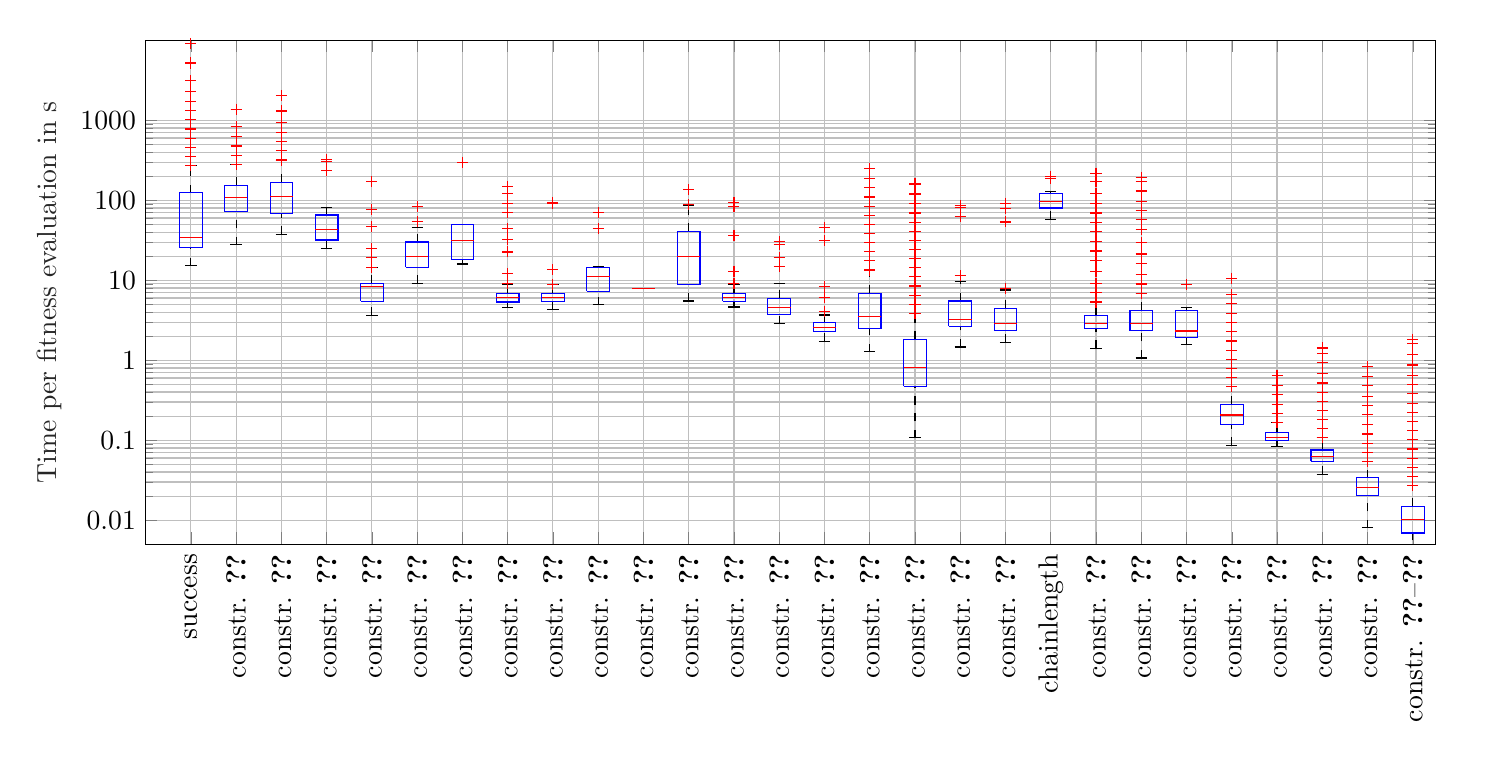
\begin{tikzpicture}

\begin{axis}[%
width=6.449in,
height=2.52in,
at={(0.496in,0.567in)},
scale only axis,
unbounded coords=jump,
xmin=0,
xmax=28.5,
xtick={1,2,3,4,5,6,7,8,9,10,11,12,13,14,15,16,17,18,19,20,21,22,23,24,25,26,27,28},
xticklabels={{success},{constr. \ref*{itm:constr_desopt}},{constr. \ref*{itm:constr_desopt}},{constr. \ref*{itm:constr_jac_traj}},{constr. \ref*{itm:constr_collinstspc_traj}},{constr. \ref*{itm:constr_collinstspc_traj}},{constr. \ref*{itm:constr_collinstspc_traj}},{constr. \ref*{itm:constr_velo}},{constr. \ref*{itm:constr_velo}},{constr. \ref*{itm:constr_prismaticcylinder_traj}},{constr. \ref*{itm:constr_prismaticcylinder_traj}},{constr. \ref*{itm:constr_jointrange_traj}},{constr. \ref*{itm:constr_jointrange_traj}},{constr. \ref*{itm:constr_iktraj}},{constr. \ref*{itm:constr_workspacecoll}},{constr. \ref*{itm:constr_installspace}},{constr. \ref*{itm:constr_selfcoll}},{constr. \ref*{itm:constr_prismaticcylinder}},{constr. \ref*{itm:constr_prismaticcylinder}},{chainlength},{constr. \ref*{itm:constr_jointrange}},{constr. \ref*{itm:constr_ik_jac}},{constr. \ref*{itm:constr_ik_jac}},{constr. \ref*{itm:constr_ik_succ}},{constr. \ref*{itm:constr_ik_succ}},{constr. \ref*{itm:constr_geom2}},{constr. \ref*{itm:constr_geom1}},{constr. \ref*{itm:constr_param_inclination}--\ref*{itm:constr_param_chainlength}}},
xticklabel style={rotate=90},
ymode=log,
ymin=0.005,
ymax=10000,
ytick={0.01,0.1,1,10,100,1000},
yticklabels={{0.01},{0.1},{1},{10},{100},{1000}},
yminorticks=true,
ylabel style={font=\color{white!15!black}},
ylabel={Time per fitness evaluation in s},
axis background/.style={fill=white},
xmajorgrids,
ymajorgrids,
yminorgrids
]
\addplot [color=black, dashed, forget plot]
  table[row sep=crcr]{%
1	123.786447\\
1	271.074828\\
};
\addplot [color=black, dashed, forget plot]
  table[row sep=crcr]{%
2	154.347325\\
2	277.335092\\
};
\addplot [color=black, dashed, forget plot]
  table[row sep=crcr]{%
3	167.25449875\\
3	313.097785\\
};
\addplot [color=black, dashed, forget plot]
  table[row sep=crcr]{%
4	65.297785\\
4	80.36201\\
};
\addplot [color=black, dashed, forget plot]
  table[row sep=crcr]{%
5	9.09887225\\
5	14.409004\\
};
\addplot [color=black, dashed, forget plot]
  table[row sep=crcr]{%
6	30.01753375\\
6	45.878832\\
};
\addplot [color=black, dashed, forget plot]
  table[row sep=crcr]{%
7	49.234908\\
7	49.234908\\
};
\addplot [color=black, dashed, forget plot]
  table[row sep=crcr]{%
8	6.770948\\
8	8.858536\\
};
\addplot [color=black, dashed, forget plot]
  table[row sep=crcr]{%
9	6.803658\\
9	8.762951\\
};
\addplot [color=black, dashed, forget plot]
  table[row sep=crcr]{%
10	14.341386\\
10	14.641265\\
};
\addplot [color=black, dashed, forget plot]
  table[row sep=crcr]{%
11	7.867104\\
11	7.867104\\
};
\addplot [color=black, dashed, forget plot]
  table[row sep=crcr]{%
12	40.368559\\
12	86.195047\\
};
\addplot [color=black, dashed, forget plot]
  table[row sep=crcr]{%
13	6.8544715\\
13	8.855427\\
};
\addplot [color=black, dashed, forget plot]
  table[row sep=crcr]{%
14	5.93691625\\
14	9.114331\\
};
\addplot [color=black, dashed, forget plot]
  table[row sep=crcr]{%
15	2.925106\\
15	3.681418\\
};
\addplot [color=black, dashed, forget plot]
  table[row sep=crcr]{%
16	6.852222\\
16	13.430652\\
};
\addplot [color=black, dashed, forget plot]
  table[row sep=crcr]{%
17	1.825502\\
17	3.857628\\
};
\addplot [color=black, dashed, forget plot]
  table[row sep=crcr]{%
18	5.5006075\\
18	9.590256\\
};
\addplot [color=black, dashed, forget plot]
  table[row sep=crcr]{%
19	4.4477085\\
19	7.561213\\
};
\addplot [color=black, dashed, forget plot]
  table[row sep=crcr]{%
20	122.180271\\
20	127.62456\\
};
\addplot [color=black, dashed, forget plot]
  table[row sep=crcr]{%
21	3.6166615\\
21	5.330132\\
};
\addplot [color=black, dashed, forget plot]
  table[row sep=crcr]{%
22	4.1684795\\
22	6.895105\\
};
\addplot [color=black, dashed, forget plot]
  table[row sep=crcr]{%
23	4.191057\\
23	4.526031\\
};
\addplot [color=black, dashed, forget plot]
  table[row sep=crcr]{%
24	0.281697\\
24	0.4684\\
};
\addplot [color=black, dashed, forget plot]
  table[row sep=crcr]{%
25	0.1246435\\
25	0.164661\\
};
\addplot [color=black, dashed, forget plot]
  table[row sep=crcr]{%
26	0.075416\\
26	0.107225\\
};
\addplot [color=black, dashed, forget plot]
  table[row sep=crcr]{%
27	0.033777\\
27	0.054247\\
};
\addplot [color=black, dashed, forget plot]
  table[row sep=crcr]{%
28	0.015011\\
28	0.027151\\
};
\addplot [color=black, dashed, forget plot]
  table[row sep=crcr]{%
1	15.102601\\
1	25.592892\\
};
\addplot [color=black, dashed, forget plot]
  table[row sep=crcr]{%
2	27.62244\\
2	71.4961565\\
};
\addplot [color=black, dashed, forget plot]
  table[row sep=crcr]{%
3	37.309894\\
3	68.232941\\
};
\addplot [color=black, dashed, forget plot]
  table[row sep=crcr]{%
4	25.053854\\
4	31.7947105\\
};
\addplot [color=black, dashed, forget plot]
  table[row sep=crcr]{%
5	3.643429\\
5	5.47933925\\
};
\addplot [color=black, dashed, forget plot]
  table[row sep=crcr]{%
6	9.210458\\
6	14.608325\\
};
\addplot [color=black, dashed, forget plot]
  table[row sep=crcr]{%
7	15.935245\\
7	18.065945\\
};
\addplot [color=black, dashed, forget plot]
  table[row sep=crcr]{%
8	4.527528\\
8	5.347809\\
};
\addplot [color=black, dashed, forget plot]
  table[row sep=crcr]{%
9	4.324491\\
9	5.409103\\
};
\addplot [color=black, dashed, forget plot]
  table[row sep=crcr]{%
10	4.915937\\
10	7.26997625\\
};
\addplot [color=black, dashed, forget plot]
  table[row sep=crcr]{%
11	7.867104\\
11	7.867104\\
};
\addplot [color=black, dashed, forget plot]
  table[row sep=crcr]{%
12	5.508612\\
12	8.859749\\
};
\addplot [color=black, dashed, forget plot]
  table[row sep=crcr]{%
13	4.627161\\
13	5.4296965\\
};
\addplot [color=black, dashed, forget plot]
  table[row sep=crcr]{%
14	2.845271\\
14	3.69286825\\
};
\addplot [color=black, dashed, forget plot]
  table[row sep=crcr]{%
15	1.707995\\
15	2.2772075\\
};
\addplot [color=black, dashed, forget plot]
  table[row sep=crcr]{%
16	1.270619\\
16	2.4665\\
};
\addplot [color=black, dashed, forget plot]
  table[row sep=crcr]{%
17	0.106743\\
17	0.4707\\
};
\addplot [color=black, dashed, forget plot]
  table[row sep=crcr]{%
18	1.463367\\
18	2.65742525\\
};
\addplot [color=black, dashed, forget plot]
  table[row sep=crcr]{%
19	1.660119\\
19	2.3507675\\
};
\addplot [color=black, dashed, forget plot]
  table[row sep=crcr]{%
20	57.058059\\
20	80.1052335\\
};
\addplot [color=black, dashed, forget plot]
  table[row sep=crcr]{%
21	1.410055\\
21	2.4693495\\
};
\addplot [color=black, dashed, forget plot]
  table[row sep=crcr]{%
22	1.065499\\
22	2.349917\\
};
\addplot [color=black, dashed, forget plot]
  table[row sep=crcr]{%
23	1.575555\\
23	1.927044\\
};
\addplot [color=black, dashed, forget plot]
  table[row sep=crcr]{%
24	0.085762\\
24	0.157222\\
};
\addplot [color=black, dashed, forget plot]
  table[row sep=crcr]{%
25	0.08368\\
25	0.097934\\
};
\addplot [color=black, dashed, forget plot]
  table[row sep=crcr]{%
26	0.037148\\
26	0.054207\\
};
\addplot [color=black, dashed, forget plot]
  table[row sep=crcr]{%
27	0.008005\\
27	0.020129\\
};
\addplot [color=black, dashed, forget plot]
  table[row sep=crcr]{%
28	0.002149\\
28	0.006917\\
};
\addplot [color=black, forget plot]
  table[row sep=crcr]{%
0.875	271.074828\\
1.125	271.074828\\
};
\addplot [color=black, forget plot]
  table[row sep=crcr]{%
1.875	277.335092\\
2.125	277.335092\\
};
\addplot [color=black, forget plot]
  table[row sep=crcr]{%
2.875	313.097785\\
3.125	313.097785\\
};
\addplot [color=black, forget plot]
  table[row sep=crcr]{%
3.875	80.36201\\
4.125	80.36201\\
};
\addplot [color=black, forget plot]
  table[row sep=crcr]{%
4.875	14.409004\\
5.125	14.409004\\
};
\addplot [color=black, forget plot]
  table[row sep=crcr]{%
5.875	45.878832\\
6.125	45.878832\\
};
\addplot [color=black, forget plot]
  table[row sep=crcr]{%
6.875	49.234908\\
7.125	49.234908\\
};
\addplot [color=black, forget plot]
  table[row sep=crcr]{%
7.875	8.858536\\
8.125	8.858536\\
};
\addplot [color=black, forget plot]
  table[row sep=crcr]{%
8.875	8.762951\\
9.125	8.762951\\
};
\addplot [color=black, forget plot]
  table[row sep=crcr]{%
9.875	14.641265\\
10.125	14.641265\\
};
\addplot [color=black, forget plot]
  table[row sep=crcr]{%
10.875	7.867104\\
11.125	7.867104\\
};
\addplot [color=black, forget plot]
  table[row sep=crcr]{%
11.875	86.195047\\
12.125	86.195047\\
};
\addplot [color=black, forget plot]
  table[row sep=crcr]{%
12.875	8.855427\\
13.125	8.855427\\
};
\addplot [color=black, forget plot]
  table[row sep=crcr]{%
13.875	9.114331\\
14.125	9.114331\\
};
\addplot [color=black, forget plot]
  table[row sep=crcr]{%
14.875	3.681418\\
15.125	3.681418\\
};
\addplot [color=black, forget plot]
  table[row sep=crcr]{%
15.875	13.430652\\
16.125	13.430652\\
};
\addplot [color=black, forget plot]
  table[row sep=crcr]{%
16.875	3.857628\\
17.125	3.857628\\
};
\addplot [color=black, forget plot]
  table[row sep=crcr]{%
17.875	9.590256\\
18.125	9.590256\\
};
\addplot [color=black, forget plot]
  table[row sep=crcr]{%
18.875	7.561213\\
19.125	7.561213\\
};
\addplot [color=black, forget plot]
  table[row sep=crcr]{%
19.875	127.62456\\
20.125	127.62456\\
};
\addplot [color=black, forget plot]
  table[row sep=crcr]{%
20.875	5.330132\\
21.125	5.330132\\
};
\addplot [color=black, forget plot]
  table[row sep=crcr]{%
21.875	6.895105\\
22.125	6.895105\\
};
\addplot [color=black, forget plot]
  table[row sep=crcr]{%
22.875	4.526031\\
23.125	4.526031\\
};
\addplot [color=black, forget plot]
  table[row sep=crcr]{%
23.875	0.4684\\
24.125	0.4684\\
};
\addplot [color=black, forget plot]
  table[row sep=crcr]{%
24.875	0.164661\\
25.125	0.164661\\
};
\addplot [color=black, forget plot]
  table[row sep=crcr]{%
25.875	0.107225\\
26.125	0.107225\\
};
\addplot [color=black, forget plot]
  table[row sep=crcr]{%
26.875	0.054247\\
27.125	0.054247\\
};
\addplot [color=black, forget plot]
  table[row sep=crcr]{%
27.875	0.027151\\
28.125	0.027151\\
};
\addplot [color=black, forget plot]
  table[row sep=crcr]{%
0.875	15.102601\\
1.125	15.102601\\
};
\addplot [color=black, forget plot]
  table[row sep=crcr]{%
1.875	27.62244\\
2.125	27.62244\\
};
\addplot [color=black, forget plot]
  table[row sep=crcr]{%
2.875	37.309894\\
3.125	37.309894\\
};
\addplot [color=black, forget plot]
  table[row sep=crcr]{%
3.875	25.053854\\
4.125	25.053854\\
};
\addplot [color=black, forget plot]
  table[row sep=crcr]{%
4.875	3.643429\\
5.125	3.643429\\
};
\addplot [color=black, forget plot]
  table[row sep=crcr]{%
5.875	9.210458\\
6.125	9.210458\\
};
\addplot [color=black, forget plot]
  table[row sep=crcr]{%
6.875	15.935245\\
7.125	15.935245\\
};
\addplot [color=black, forget plot]
  table[row sep=crcr]{%
7.875	4.527528\\
8.125	4.527528\\
};
\addplot [color=black, forget plot]
  table[row sep=crcr]{%
8.875	4.324491\\
9.125	4.324491\\
};
\addplot [color=black, forget plot]
  table[row sep=crcr]{%
9.875	4.915937\\
10.125	4.915937\\
};
\addplot [color=black, forget plot]
  table[row sep=crcr]{%
10.875	7.867104\\
11.125	7.867104\\
};
\addplot [color=black, forget plot]
  table[row sep=crcr]{%
11.875	5.508612\\
12.125	5.508612\\
};
\addplot [color=black, forget plot]
  table[row sep=crcr]{%
12.875	4.627161\\
13.125	4.627161\\
};
\addplot [color=black, forget plot]
  table[row sep=crcr]{%
13.875	2.845271\\
14.125	2.845271\\
};
\addplot [color=black, forget plot]
  table[row sep=crcr]{%
14.875	1.707995\\
15.125	1.707995\\
};
\addplot [color=black, forget plot]
  table[row sep=crcr]{%
15.875	1.270619\\
16.125	1.270619\\
};
\addplot [color=black, forget plot]
  table[row sep=crcr]{%
16.875	0.106743\\
17.125	0.106743\\
};
\addplot [color=black, forget plot]
  table[row sep=crcr]{%
17.875	1.463367\\
18.125	1.463367\\
};
\addplot [color=black, forget plot]
  table[row sep=crcr]{%
18.875	1.660119\\
19.125	1.660119\\
};
\addplot [color=black, forget plot]
  table[row sep=crcr]{%
19.875	57.058059\\
20.125	57.058059\\
};
\addplot [color=black, forget plot]
  table[row sep=crcr]{%
20.875	1.410055\\
21.125	1.410055\\
};
\addplot [color=black, forget plot]
  table[row sep=crcr]{%
21.875	1.065499\\
22.125	1.065499\\
};
\addplot [color=black, forget plot]
  table[row sep=crcr]{%
22.875	1.575555\\
23.125	1.575555\\
};
\addplot [color=black, forget plot]
  table[row sep=crcr]{%
23.875	0.085762\\
24.125	0.085762\\
};
\addplot [color=black, forget plot]
  table[row sep=crcr]{%
24.875	0.08368\\
25.125	0.08368\\
};
\addplot [color=black, forget plot]
  table[row sep=crcr]{%
25.875	0.037148\\
26.125	0.037148\\
};
\addplot [color=black, forget plot]
  table[row sep=crcr]{%
26.875	0.008005\\
27.125	0.008005\\
};
\addplot [color=black, forget plot]
  table[row sep=crcr]{%
27.875	0.002149\\
28.125	0.002149\\
};
\addplot [color=blue, forget plot]
  table[row sep=crcr]{%
0.75	25.592892\\
0.75	123.786447\\
1.25	123.786447\\
1.25	25.592892\\
0.75	25.592892\\
};
\addplot [color=blue, forget plot]
  table[row sep=crcr]{%
1.75	71.4961565\\
1.75	154.347325\\
2.25	154.347325\\
2.25	71.4961565\\
1.75	71.4961565\\
};
\addplot [color=blue, forget plot]
  table[row sep=crcr]{%
2.75	68.232941\\
2.75	167.25449875\\
3.25	167.25449875\\
3.25	68.232941\\
2.75	68.232941\\
};
\addplot [color=blue, forget plot]
  table[row sep=crcr]{%
3.75	31.7947105\\
3.75	65.297785\\
4.25	65.297785\\
4.25	31.7947105\\
3.75	31.7947105\\
};
\addplot [color=blue, forget plot]
  table[row sep=crcr]{%
4.75	5.47933925\\
4.75	9.09887225\\
5.25	9.09887225\\
5.25	5.47933925\\
4.75	5.47933925\\
};
\addplot [color=blue, forget plot]
  table[row sep=crcr]{%
5.75	14.608325\\
5.75	30.01753375\\
6.25	30.01753375\\
6.25	14.608325\\
5.75	14.608325\\
};
\addplot [color=blue, forget plot]
  table[row sep=crcr]{%
6.75	18.065945\\
6.75	49.234908\\
7.25	49.234908\\
7.25	18.065945\\
6.75	18.065945\\
};
\addplot [color=blue, forget plot]
  table[row sep=crcr]{%
7.75	5.347809\\
7.75	6.770948\\
8.25	6.770948\\
8.25	5.347809\\
7.75	5.347809\\
};
\addplot [color=blue, forget plot]
  table[row sep=crcr]{%
8.75	5.409103\\
8.75	6.803658\\
9.25	6.803658\\
9.25	5.409103\\
8.75	5.409103\\
};
\addplot [color=blue, forget plot]
  table[row sep=crcr]{%
9.75	7.26997625\\
9.75	14.341386\\
10.25	14.341386\\
10.25	7.26997625\\
9.75	7.26997625\\
};
\addplot [color=blue, forget plot]
  table[row sep=crcr]{%
10.75	7.867104\\
10.75	7.867104\\
11.25	7.867104\\
11.25	7.867104\\
10.75	7.867104\\
};
\addplot [color=blue, forget plot]
  table[row sep=crcr]{%
11.75	8.859749\\
11.75	40.368559\\
12.25	40.368559\\
12.25	8.859749\\
11.75	8.859749\\
};
\addplot [color=blue, forget plot]
  table[row sep=crcr]{%
12.75	5.4296965\\
12.75	6.8544715\\
13.25	6.8544715\\
13.25	5.4296965\\
12.75	5.4296965\\
};
\addplot [color=blue, forget plot]
  table[row sep=crcr]{%
13.75	3.69286825\\
13.75	5.93691625\\
14.25	5.93691625\\
14.25	3.69286825\\
13.75	3.69286825\\
};
\addplot [color=blue, forget plot]
  table[row sep=crcr]{%
14.75	2.2772075\\
14.75	2.925106\\
15.25	2.925106\\
15.25	2.2772075\\
14.75	2.2772075\\
};
\addplot [color=blue, forget plot]
  table[row sep=crcr]{%
15.75	2.4665\\
15.75	6.852222\\
16.25	6.852222\\
16.25	2.4665\\
15.75	2.4665\\
};
\addplot [color=blue, forget plot]
  table[row sep=crcr]{%
16.75	0.4707\\
16.75	1.825502\\
17.25	1.825502\\
17.25	0.4707\\
16.75	0.4707\\
};
\addplot [color=blue, forget plot]
  table[row sep=crcr]{%
17.75	2.65742525\\
17.75	5.5006075\\
18.25	5.5006075\\
18.25	2.65742525\\
17.75	2.65742525\\
};
\addplot [color=blue, forget plot]
  table[row sep=crcr]{%
18.75	2.3507675\\
18.75	4.4477085\\
19.25	4.4477085\\
19.25	2.3507675\\
18.75	2.3507675\\
};
\addplot [color=blue, forget plot]
  table[row sep=crcr]{%
19.75	80.1052335\\
19.75	122.180271\\
20.25	122.180271\\
20.25	80.1052335\\
19.75	80.1052335\\
};
\addplot [color=blue, forget plot]
  table[row sep=crcr]{%
20.75	2.4693495\\
20.75	3.6166615\\
21.25	3.6166615\\
21.25	2.4693495\\
20.75	2.4693495\\
};
\addplot [color=blue, forget plot]
  table[row sep=crcr]{%
21.75	2.349917\\
21.75	4.1684795\\
22.25	4.1684795\\
22.25	2.349917\\
21.75	2.349917\\
};
\addplot [color=blue, forget plot]
  table[row sep=crcr]{%
22.75	1.927044\\
22.75	4.191057\\
23.25	4.191057\\
23.25	1.927044\\
22.75	1.927044\\
};
\addplot [color=blue, forget plot]
  table[row sep=crcr]{%
23.75	0.157222\\
23.75	0.281697\\
24.25	0.281697\\
24.25	0.157222\\
23.75	0.157222\\
};
\addplot [color=blue, forget plot]
  table[row sep=crcr]{%
24.75	0.097934\\
24.75	0.1246435\\
25.25	0.1246435\\
25.25	0.097934\\
24.75	0.097934\\
};
\addplot [color=blue, forget plot]
  table[row sep=crcr]{%
25.75	0.054207\\
25.75	0.075416\\
26.25	0.075416\\
26.25	0.054207\\
25.75	0.054207\\
};
\addplot [color=blue, forget plot]
  table[row sep=crcr]{%
26.75	0.020129\\
26.75	0.033777\\
27.25	0.033777\\
27.25	0.020129\\
26.75	0.020129\\
};
\addplot [color=blue, forget plot]
  table[row sep=crcr]{%
27.75	0.006917\\
27.75	0.015011\\
28.25	0.015011\\
28.25	0.006917\\
27.75	0.006917\\
};
\addplot [color=red, forget plot]
  table[row sep=crcr]{%
0.75	34.1471385\\
1.25	34.1471385\\
};
\addplot [color=red, forget plot]
  table[row sep=crcr]{%
1.75	107.984888\\
2.25	107.984888\\
};
\addplot [color=red, forget plot]
  table[row sep=crcr]{%
2.75	112.519567\\
3.25	112.519567\\
};
\addplot [color=red, forget plot]
  table[row sep=crcr]{%
3.75	42.9711515\\
4.25	42.9711515\\
};
\addplot [color=red, forget plot]
  table[row sep=crcr]{%
4.75	8.268415\\
5.25	8.268415\\
};
\addplot [color=red, forget plot]
  table[row sep=crcr]{%
5.75	19.827957\\
6.25	19.827957\\
};
\addplot [color=red, forget plot]
  table[row sep=crcr]{%
6.75	31.3085815\\
7.25	31.3085815\\
};
\addplot [color=red, forget plot]
  table[row sep=crcr]{%
7.75	6.042387\\
8.25	6.042387\\
};
\addplot [color=red, forget plot]
  table[row sep=crcr]{%
8.75	6.0866835\\
9.25	6.0866835\\
};
\addplot [color=red, forget plot]
  table[row sep=crcr]{%
9.75	11.190725\\
10.25	11.190725\\
};
\addplot [color=red, forget plot]
  table[row sep=crcr]{%
10.75	7.867104\\
11.25	7.867104\\
};
\addplot [color=red, forget plot]
  table[row sep=crcr]{%
11.75	19.7779065\\
12.25	19.7779065\\
};
\addplot [color=red, forget plot]
  table[row sep=crcr]{%
12.75	6.113933\\
13.25	6.113933\\
};
\addplot [color=red, forget plot]
  table[row sep=crcr]{%
13.75	4.525064\\
14.25	4.525064\\
};
\addplot [color=red, forget plot]
  table[row sep=crcr]{%
14.75	2.554502\\
15.25	2.554502\\
};
\addplot [color=red, forget plot]
  table[row sep=crcr]{%
15.75	3.527561\\
16.25	3.527561\\
};
\addplot [color=red, forget plot]
  table[row sep=crcr]{%
16.75	0.816999\\
17.25	0.816999\\
};
\addplot [color=red, forget plot]
  table[row sep=crcr]{%
17.75	3.266164\\
18.25	3.266164\\
};
\addplot [color=red, forget plot]
  table[row sep=crcr]{%
18.75	2.895795\\
19.25	2.895795\\
};
\addplot [color=red, forget plot]
  table[row sep=crcr]{%
19.75	97.003035\\
20.25	97.003035\\
};
\addplot [color=red, forget plot]
  table[row sep=crcr]{%
20.75	2.912858\\
21.25	2.912858\\
};
\addplot [color=red, forget plot]
  table[row sep=crcr]{%
21.75	2.8717145\\
22.25	2.8717145\\
};
\addplot [color=red, forget plot]
  table[row sep=crcr]{%
22.75	2.322527\\
23.25	2.322527\\
};
\addplot [color=red, forget plot]
  table[row sep=crcr]{%
23.75	0.206886\\
24.25	0.206886\\
};
\addplot [color=red, forget plot]
  table[row sep=crcr]{%
24.75	0.10675\\
25.25	0.10675\\
};
\addplot [color=red, forget plot]
  table[row sep=crcr]{%
25.75	0.0630445\\
26.25	0.0630445\\
};
\addplot [color=red, forget plot]
  table[row sep=crcr]{%
26.75	0.025934\\
27.25	0.025934\\
};
\addplot [color=red, forget plot]
  table[row sep=crcr]{%
27.75	0.010296\\
28.25	0.010296\\
};
\addplot [color=black, only marks, mark=+, mark options={solid, draw=red}, forget plot]
  table[row sep=crcr]{%
1	271.078109\\
1	352.421981\\
1	458.30276\\
1	595.939549\\
1	776.998656\\
1	1010.709355\\
1	1328.666596\\
1	1730.959515\\
1	2264.6653\\
1	3117.685149\\
1	5196.786853\\
1	9146.318036\\
};
\addplot [color=black, only marks, mark=+, mark options={solid, draw=red}, forget plot]
  table[row sep=crcr]{%
2	279.856683\\
2	366.752712\\
2	477.112975\\
2	628.909301\\
2	831.798361\\
2	1349.86609\\
2	1375.419227\\
};
\addplot [color=black, only marks, mark=+, mark options={solid, draw=red}, forget plot]
  table[row sep=crcr]{%
3	318.405353\\
3	415.310058\\
3	542.668544\\
3	708.086027\\
3	948.18956\\
3	1305.810499\\
3	2048.918539\\
};
\addplot [color=black, only marks, mark=+, mark options={solid, draw=red}, forget plot]
  table[row sep=crcr]{%
4	234.919049\\
4	308.154177\\
4	320.272458\\
};
\addplot [color=black, only marks, mark=+, mark options={solid, draw=red}, forget plot]
  table[row sep=crcr]{%
5	14.545025\\
5	19.057092\\
5	25.203607\\
5	46.378056\\
5	77.318439\\
5	169.613583\\
};
\addplot [color=black, only marks, mark=+, mark options={solid, draw=red}, forget plot]
  table[row sep=crcr]{%
6	53.930537\\
6	82.461856\\
};
\addplot [color=black, only marks, mark=+, mark options={solid, draw=red}, forget plot]
  table[row sep=crcr]{%
7	298.699656\\
};
\addplot [color=black, only marks, mark=+, mark options={solid, draw=red}, forget plot]
  table[row sep=crcr]{%
8	9.135066\\
8	11.994717\\
8	22.567487\\
8	32.026793\\
8	44.400364\\
8	70.678086\\
8	92.19582\\
8	121.146369\\
8	146.904329\\
};
\addplot [color=black, only marks, mark=+, mark options={solid, draw=red}, forget plot]
  table[row sep=crcr]{%
9	8.956132\\
9	13.480079\\
9	90.711184\\
9	93.681337\\
};
\addplot [color=black, only marks, mark=+, mark options={solid, draw=red}, forget plot]
  table[row sep=crcr]{%
10	43.927161\\
10	70.267663\\
};
\addplot [color=black, only marks, mark=+, mark options={solid, draw=red}, forget plot]
  table[row sep=crcr]{%
nan	nan\\
};
\addplot [color=black, only marks, mark=+, mark options={solid, draw=red}, forget plot]
  table[row sep=crcr]{%
12	88.368955\\
12	134.620493\\
};
\addplot [color=black, only marks, mark=+, mark options={solid, draw=red}, forget plot]
  table[row sep=crcr]{%
13	9.085692\\
13	13.019501\\
13	36.601829\\
13	84.074043\\
13	93.947386\\
};
\addplot [color=black, only marks, mark=+, mark options={solid, draw=red}, forget plot]
  table[row sep=crcr]{%
14	14.933917\\
14	19.421108\\
14	27.621206\\
14	30.272053\\
};
\addplot [color=black, only marks, mark=+, mark options={solid, draw=red}, forget plot]
  table[row sep=crcr]{%
15	4.098754\\
15	6.152144\\
15	8.308653\\
15	31.516832\\
15	46.073932\\
};
\addplot [color=black, only marks, mark=+, mark options={solid, draw=red}, forget plot]
  table[row sep=crcr]{%
16	13.431123\\
16	17.463061\\
16	22.704365\\
16	29.516442\\
16	38.374283\\
16	49.898962\\
16	64.874384\\
16	84.354762\\
16	109.723298\\
16	142.734211\\
16	185.884174\\
16	250.803122\\
};
\addplot [color=black, only marks, mark=+, mark options={solid, draw=red}, forget plot]
  table[row sep=crcr]{%
17	3.857736\\
17	5.015174\\
17	6.519734\\
17	8.47613\\
17	11.020519\\
17	14.327557\\
17	18.626842\\
17	24.220807\\
17	31.501566\\
17	40.955365\\
17	53.242779\\
17	69.27933\\
17	90.091647\\
17	119.780563\\
17	158.491096\\
17	162.379267\\
};
\addplot [color=black, only marks, mark=+, mark options={solid, draw=red}, forget plot]
  table[row sep=crcr]{%
18	11.3422\\
18	62.411237\\
18	81.52526\\
18	85.853589\\
};
\addplot [color=black, only marks, mark=+, mark options={solid, draw=red}, forget plot]
  table[row sep=crcr]{%
19	7.782762\\
19	53.521119\\
19	78.227987\\
19	92.192788\\
};
\addplot [color=black, only marks, mark=+, mark options={solid, draw=red}, forget plot]
  table[row sep=crcr]{%
20	187.381133\\
20	198.370046\\
};
\addplot [color=black, only marks, mark=+, mark options={solid, draw=red}, forget plot]
  table[row sep=crcr]{%
21	5.345269\\
21	6.95057\\
21	9.03665\\
21	12.856193\\
21	17.753034\\
21	23.229282\\
21	30.336197\\
21	40.851434\\
21	53.272551\\
21	69.288468\\
21	90.266323\\
21	122.874625\\
21	169.927749\\
21	218.528757\\
};
\addplot [color=black, only marks, mark=+, mark options={solid, draw=red}, forget plot]
  table[row sep=crcr]{%
22	6.896658\\
22	8.965898\\
22	11.661467\\
22	16.299648\\
22	21.287851\\
22	29.538094\\
22	43.203421\\
22	57.41653\\
22	75.063658\\
22	97.677503\\
22	130.622795\\
22	173.732205\\
22	193.319214\\
};
\addplot [color=black, only marks, mark=+, mark options={solid, draw=red}, forget plot]
  table[row sep=crcr]{%
23	8.799476\\
};
\addplot [color=black, only marks, mark=+, mark options={solid, draw=red}, forget plot]
  table[row sep=crcr]{%
24	0.46841\\
24	0.60899\\
24	0.791759\\
24	1.029318\\
24	1.338206\\
24	1.740593\\
24	2.263252\\
24	2.951134\\
24	3.886721\\
24	5.110682\\
24	6.675241\\
24	10.61063\\
};
\addplot [color=black, only marks, mark=+, mark options={solid, draw=red}, forget plot]
  table[row sep=crcr]{%
25	0.164744\\
25	0.215319\\
25	0.28247\\
25	0.370143\\
25	0.487234\\
25	0.643632\\
};
\addplot [color=black, only marks, mark=+, mark options={solid, draw=red}, forget plot]
  table[row sep=crcr]{%
26	0.107234\\
26	0.139409\\
26	0.18125\\
26	0.235677\\
26	0.306838\\
26	0.399505\\
26	0.519692\\
26	0.688134\\
26	0.939355\\
26	1.221615\\
26	1.420865\\
};
\addplot [color=black, only marks, mark=+, mark options={solid, draw=red}, forget plot]
  table[row sep=crcr]{%
27	0.054258\\
27	0.070561\\
27	0.091737\\
27	0.11953\\
27	0.156528\\
27	0.206944\\
27	0.270097\\
27	0.35309\\
27	0.480275\\
27	0.627522\\
27	0.844434\\
};
\addplot [color=black, only marks, mark=+, mark options={solid, draw=red}, forget plot]
  table[row sep=crcr]{%
28	0.027153\\
28	0.035299\\
28	0.045891\\
28	0.059664\\
28	0.077702\\
28	0.101094\\
28	0.131586\\
28	0.171292\\
28	0.222751\\
28	0.290282\\
28	0.37888\\
28	0.496756\\
28	0.64963\\
28	0.871419\\
28	1.190338\\
28	1.623173\\
28	1.835289\\
};
\end{axis}

\begin{axis}[%
width=7.087in,
height=3.15in,
at={(0in,0in)},
scale only axis,
xmin=0,
xmax=1,
ymin=0,
ymax=1,
axis line style={draw=none},
ticks=none,
axis x line*=bottom,
axis y line*=left
]
\end{axis}
\end{tikzpicture}%
  \end{adjustwidth}
  \caption{Computation
    time of the fitness function (logarithmic scale) in relation to the number of the violated constraint (from Section~\ref{sec:ds_constraints}) that led to abortion. The class ``chainlength'' comes from checking if the length of a leg chain that includes a prismatic joint exceeds the maximum allowed length. Outlier markers were thinned out (193 of 97 k left over) to increase visibility of the data. Duplicate constraints result from multiple similar checks, e.g., for different Jacobian matrices in constraint~\ref*{itm:constr_ik_jac}.}
  \label{fig:computation_time}
\end{figure}


One parameterization is chosen for each of the valid parallel robots from the \propername{Pareto} diagrams.
The selection is based on the \propername{Pareto} diagram of collision distance vs. actuator power in Figure~\ref{fig:lufipkm_pareto_power_mass_groups}. 
Both criteria are normalized to their best-achieved values (for all structures), and the best particle for equal weighting is chosen to illustrate the results' appearance.
The performance values and kinematic parameters of these reference solutions are summarized in Table~\ref{tab:lufipkm_results_pris} for prismatic and Table~\ref{tab:lufipkm_results_rev} for revolute actuation.
Kinematic sketches are given in Figures~\ref{fig:lufipkm_robots2}--\ref{fig:lufipkm_robots4}.

\begin{table}[H]
  \caption{Summary
    of one typical particle for each robot with \emph{prismatic actuation}, visualized in Figures~\ref{fig:lufipkm_robots2} and \ref{fig:lufipkm_robots3}. Abbreviations: ``coll.'' (collision distance), ``velo.'' (actuator velocity), ``cond.'' (largest \propername{Jacobian} condition number), $n$ (number of optimization variables), $r_\mathrm{b}$ (base radius), $d_\mathrm{b}$ (base-joint pair distance), $\gamma_\mathrm{b}$ (base-joint inclination), $r_\mathrm{p}$ (platform radius), $d_\mathrm{p}$ (platform-joint pair distance), $e_\mathrm{link}$ (material strength of the links), $d_\mathrm{link}$ (diameter of the links), ``Eng. Sol.'' engineering solution. Continued horizontally in Table~\ref{tab:lufipkm_results_pris_dh}.}
  \begin{adjustwidth}{-\extralength}{0cm}
    \centering
    \label{tab:lufipkm_results_pris}
    \begin{tabularx}{\fulllength}{lRRRRRRRRRRRRR} %
      \toprule
      \multicolumn{1}{c}{\textbf{Robot}}
      & \multicolumn{5}{c}{\textbf{Performance}} & \multicolumn{8}{c}{\textbf{Kinematic and Design Parameters}} \\
      \midrule
      & \multicolumn{1}{r}{coll.} & \multicolumn{1}{r}{power} & \multicolumn{1}{r}{force} & \multicolumn{1}{r}{velo.} & \multicolumn{1}{r}{cond.} &  \multicolumn{1}{c}{$n$} &
      \multicolumn{1}{c}{$r_\mathrm{b}$} & \multicolumn{1}{c}{$d_\mathrm{b}$} & \multicolumn{1}{c}{$\gamma_\mathrm{b}$} & \multicolumn{1}{c}{$r_\mathrm{p}$}& \multicolumn{1}{c}{$d_\mathrm{p}$} & \multicolumn{1}{c}{$e_\mathrm{link}$} & \multicolumn{1}{c}{$d_\mathrm{link}$} \\
      & \multicolumn{1}{c}{mm} & \multicolumn{1}{c}{kW} & \multicolumn{1}{c}{kN} & \multicolumn{1}{c}{m/s} & \multicolumn{1}{c}{} & & \multicolumn{1}{c}{mm} & \multicolumn{1}{c}{mm} & \multicolumn{1}{c}{deg} & \multicolumn{1}{c}{mm} & \multicolumn{1}{c}{mm} & \multicolumn{1}{c}{mm} & \multicolumn{1}{c}{mm} \\
      \midrule %
      \hyperrefl{restabrow:P6PRRRRR4V2GxPxA1}{6-\underline{P}{R}{U}{U}},\,C-R & 18 & 1.15 & 2.17 & 0.53 & 25 & 16 & 613 & 219 & 37 & 165 & 346 & 11 & 27 \\ % group 1; lufipkm_20230413_Diss_processworkspace_allrob_default/Rob454_P6PRRRRR4V2G8P6A1 (Pareto-Index 1)
\hyperrefl{restabrow:P6PRRRRR4V3GxPxA1}{6-\underline{P}{R}{R}{R}{U}},\,V-R & 0 & 1.45 & 2.73 & 0.53 & 24 & 17 & 495 & 618 & 0 & 212 & 219 & 10 & 40 \\ % group 2; lufipkm_20230418_Diss_processworkspace_robotsfrom0415_default2/Rob21_P6PRRRRR4V3G5P6A1 (Pareto-Index 1)
\midrule
\hyperrefl{restabrow:P6PRRRRR6GxPxA1}{6-\underline{P}{R}{R}{R}{R}{R}},\,C-T & 10 & 1.82 & 3.47 & 0.52 & 50 & 21 & 410 & 255 & 173 & 152 & 275 & 14 & 31 \\ % group 3; lufipkm_20230418_Diss_processworkspace_robotsfrom0415_default2/Rob23_P6PRRRRR6G8P5A1 (Pareto-Index 1)
\hyperrefl{restabrow:P6PRRRRR6V2GxPxA1}{6-\underline{P}{R}{R}{S}},\,V-V & 69 & 1.62 & 2.89 & 0.56 & 23 & 16 & 551 & 254 & 0 & 194 & 273 & 10 & 36 \\ % group 4; lufipkm_20230413_Diss_processworkspace_allrob_default/Rob686_P6PRRRRR6V2G5P4A1 (Pareto-Index 3)
\hyperrefl{restabrow:P6PRRRRR6V4GxPxA1}{6-\underline{P}{U}{S}},\,V-V & 35 & 1.28 & 2.46 & 0.52 & 23 & 13 & 534 & 257 & 0 & 174 & 320 & 4 & 33 \\ % group 5; lufipkm_20230413_Diss_processworkspace_allrob_default/Rob706_P6PRRRRR6V4G5P4A1 (Pareto-Index 5)
\midrule
\hyperrefl{restabrow:P6RPRRRR10V5GxPxA2}{6-{R}\underline{P}{U}{U}},\,R-R & 69 & 1.42 & 3.03 & 0.47 & 25 & 13 & 722 & 159 & 0 & 183 & 287 & 12 & 32 \\ % group 6; lufipkm_20230413_Diss_processworkspace_allrob_default/Rob840_P6RPRRRR10V5G7P6A1 (Pareto-Index 9)
\hyperrefl{restabrow:P6RPRRRR10V6GxPxA2}{6-{R}\underline{P}{R}{R}{U}},\,C-R & 14 & 1.94 & 4.06 & 0.48 & 30 & 16 & 536 & 269 & 33 & 210 & 233 & 10 & 37 \\ % group 7; lufipkm_20230418_Diss_processworkspace_robotsfrom0415_default2/Rob62_P6RPRRRR10V6G8P6A1 (Pareto-Index 2)
\midrule
\hyperrefl{restabrow:P6RPRRRR12V4GxPxA2}{6-{R}\underline{P}{R}{R}{R}{R}},\,C-c & 11 & 2.57 & 5.92 & 0.43 & 116 & 19 & 419 & 146 & 10 & 148 & \multicolumn{1}{c}{---} & 18 & 43 \\ % group 8; lufipkm_20230418_Diss_processworkspace_robotsfrom0415_default2/Rob63_P6RPRRRR12V4G8P9A1 (Pareto-Index 1)
\hyperrefl{restabrow:P6RPRRRR12V5GxPxA2}{6-{R}\underline{P}{R}{S}},\,C-V & 27 & 1.47 & 2.84 & 0.52 & 20 & 15 & 407 & 126 & 83 & 166 & 297 & 10 & 36 \\ % group 9; lufipkm_20230413_Diss_processworkspace_allrob_default/Rob1090_P6RPRRRR12V5G8P4A1 (Pareto-Index 1)
\midrule
\hyperrefl{restabrow:P6RRPRRR4V5GxPxA3}{6-{R}{R}\underline{P}{R}{U} var. 1},\,T-T & 2 & 1.43 & 2.66 & 0.54 & 31 & 14 & 502 & 203 & 0 & 157 & 305 & 19 & 38 \\ % group 10; lufipkm_20230418_Diss_processworkspace_robotsfrom0415_default2/Rob158_P6RRPRRR4V5G6P5A1 (Pareto-Index 1)
\hyperrefl{restabrow:P6RRPRRR4V6GxPxA3}{6-{U}\underline{P}{R}{U} var. 1},\,T-T & 25 & 1.06 & 2.06 & 0.52 & 17 & 11 & 691 & 196 & 0 & 171 & 330 & 15 & 33 \\ % group 11; lufipkm_20230413_Diss_processworkspace_allrob_default/Rob2430_P6RRPRRR4V6G6P5A1 (Pareto-Index 1)
\midrule
\hyperrefl{restabrow:P6RRPRRR5V6GxPxA3}{6-{U}\underline{P}{U}{R} var. 1},\,R-T & 35 & 3.73 & 3.08 & 1.21 & 21 & 11 & 403 & 1112 & 0 & 216 & 186 & 8 & 46 \\ % group 12; lufipkm_20230413_Diss_processworkspace_allrob_default/Rob2650_P6RRPRRR5V6G7P5A1 (Pareto-Index 2)
\midrule
\hyperrefl{restabrow:P6RRPRRR7V5GxPxA3}{6-{U}\underline{P}{U}{R} var. 2},\,V-T & 3 & 1.87 & 2.61 & 0.71 & 34 & 10 & 401 & 80 & 0 & 176 & 326 & 18 & 43 \\ % group 13; lufipkm_20230413_Diss_processworkspace_allrob_default/Rob2770_P6RRPRRR7V5G5P5A1 (Pareto-Index 1)
\hyperrefl{restabrow:P6RRPRRR7V6GxPxA3}{6-{R}{R}\underline{P}{U}{R}},\,C-R & 11 & 1.99 & 3.19 & 0.62 & 35 & 13 & 398 & 203 & 14 & 191 & 275 & 20 & 49 \\ % group 14; lufipkm_20230418_Diss_processworkspace_robotsfrom0415_default2/Rob173_P6RRPRRR7V6G8P6A1 (Pareto-Index 1)
\midrule
\hyperrefl{restabrow:P6RRPRRR12V4GxPxA3}{6-{R}{R}\underline{P}{R}{U} var. 2},\,V-T & 25 & 1.32 & 2.69 & 0.49 & 19 & 13 & 411 & 230 & 0 & 177 & 324 & 10 & 40 \\ % group 15; lufipkm_20230418_Diss_processworkspace_robotsfrom0415_default2/Rob77_P6RRPRRR12V4G5P5A1 (Pareto-Index 1)
\hyperrefl{restabrow:P6RRPRRR12V5GxPxA3}{6-{U}\underline{P}{R}{U} var. 3},\,C-T & 48 & 1.41 & 2.93 & 0.48 & 37 & 11 & 470 & 237 & 14 & 170 & 289 & 16 & 32 \\ % group 16; lufipkm_20230413_Diss_processworkspace_allrob_default/Rob1843_P6RRPRRR12V5G8P5A1 (Pareto-Index 4)
\hyperrefl{restabrow:P6RRPRRR12V6GxPxA3}{6-{R}{R}\underline{P}{\`R}{\`R}{R}},\,V-T & 10 & 1.76 & 3.31 & 0.53 & 35 & 15 & 408 & 217 & 0 & 164 & 243 & 16 & 43 \\ % group 17; lufipkm_20230417_Diss_processworkspace_robotsfrom0415_default2/Rob31_P6RRPRRR12V6G5P5A1 (Pareto-Index 1)
\midrule
\hyperrefl{restabrow:P6RRPRRR14V5GxPxA3}{6-{R}{R}\underline{P}{S}},\,T-v & 113 & 1.43 & 3.05 & 0.47 & 28 & 13 & 398 & 1097 & 0 & 231 & \multicolumn{1}{c}{---} & 1 & 39 \\ % group 18; lufipkm_20230413_Diss_processworkspace_allrob_default/Rob2149_P6RRPRRR14V5G6P1A1 (Pareto-Index 1)
\hyperrefl{restabrow:P6RRPRRR14V6GxPxA3}{6-{U}\underline{P}{S}},\,T-V & 155 & 1.24 & 2.64 & 0.47 & 21 & 11 & 399 & 1219 & 0 & 212 & 226 & 1 & 13 \\ % group 19; lufipkm_20230418_Diss_processworkspace_robotsfrom0415_default2/Rob115_P6RRPRRR14V6G6P4A1 (Pareto-Index 26)
\hyperrefl{restabrow:P6RRPRRR14V7GxPxA3}{6-{R}{R}\underline{P}{R}{R}{R}},\,R-R & 50 & 1.10 & 1.30 & 0.85 & 15 & 18 & 408 & 1069 & 0 & 184 & 201 & 1 & 36 \\ % group 20; lufipkm_20230418_Diss_processworkspace_robotsfrom0415_default2/Rob145_P6RRPRRR14V7G7P6A1 (Pareto-Index 2)
\midrule
\hyperrefl{restabrow:P6RRRPRR9V6GxPxA4}{6-{R}{R}{R}\underline{P}{U} var. 1},\,C-R & 55 & 1.27 & 2.69 & 0.47 & 32 & 16 & 406 & 154 & 72 & 185 & 274 & 3 & 35 \\ % group 21; lufipkm_20230418_Diss_processworkspace_robotsfrom0415_default2/Rob494_P6RRRPRR9V6G8P6A1 (Pareto-Index 2)
\hyperrefl{restabrow:P6RRRPRR9V7GxPxA4}{6-{R}{U}\underline{P}{U} var. 1},\,C-T & 74 & 1.27 & 2.47 & 0.51 & 28 & 13 & 615 & 186 & 111 & 181 & 308 & 1 & 23 \\ % group 22; lufipkm_20230418_Diss_processworkspace_robotsfrom0415_default2/Rob545_P6RRRPRR9V7G8P5A1 (Pareto-Index 4)
\hyperrefl{restabrow:P6RRRPRR9V8GxPxA4}{6-{U}{R}\underline{P}{U} var. 1},\,V-R & 74 & 1.15 & 2.40 & 0.48 & 26 & 12 & 557 & 111 & 0 & 171 & 306 & 1 & 14 \\ % group 23; lufipkm_20230413_Diss_processworkspace_allrob_default/Rob4916_P6RRRPRR9V8G5P6A1 (Pareto-Index 3)
\hyperrefl{restabrow:P6RRRPRR9V9GxPxA4}{6-{S}\underline{P}{U}},\,V-T & 84 & 1.15 & 2.31 & 0.50 & 23 & 8 & 651 & 130 & 0 & 175 & 301 & 1 & 13 \\ % group 24; lufipkm_20230418_Diss_processworkspace_robotsfrom0415_default2/Rob605_P6RRRPRR9V9G5P5A1 (Pareto-Index 6)
\hyperrefl{restabrow:P6RRRPRR9V10GxPxA4}{6-{\`R}{R}{\'R}\underline{\'P}{R}{\`R}},\,R-V & 64 & 1.39 & 3.01 & 0.46 & 25 & 17 & 700 & 219 & 0 & 176 & 273 & 7 & 31 \\ % group 25; lufipkm_20230418_Diss_processworkspace_robotsfrom0415_default2/Rob438_P6RRRPRR9V10G7P4A1 (Pareto-Index 1)
\midrule
\hyperrefl{restabrow:P6RRRPRR11V5GxPxA4}{6-{R}{U}\underline{P}{U} var. 2},\,T-T & 76 & 1.29 & 2.77 & 0.46 & 23 & 11 & 725 & 225 & 0 & 188 & 292 & 1 & 32 \\ % group 26; lufipkm_20230413_Diss_processworkspace_allrob_default/Rob3118_P6RRRPRR11V5G6P5A1 (Pareto-Index 7)
\hyperrefl{restabrow:P6RRRPRR11V6GxPxA4}{6-{R}{R}{R}\underline{P}{U} var. 2},\,C-t & 42 & 1.33 & 3.03 & 0.44 & 17 & 13 & 399 & 660 & 45 & 185 & \multicolumn{1}{c}{---} & 15 & 30 \\ % group 27; lufipkm_20230413_Diss_processworkspace_allrob_default/Rob3203_P6RRRPRR11V6G8P2A1 (Pareto-Index 2)
\hyperrefl{restabrow:P6RRRPRR11V8GxPxA4}{6-{R}{R}{\`R}\underline{P}{\`R}{R}},\,C-R & 49 & 1.15 & 1.64 & 0.70 & 15 & 16 & 428 & 807 & 81 & 161 & 198 & 3 & 35 \\ % group 28; lufipkm_20230413_Diss_processworkspace_allrob_default/Rob3279_P6RRRPRR11V8G8P6A1 (Pareto-Index 3)
\midrule
\hyperrefl{restabrow:P6RRRPRR15V6GxPxA4}{6-{R}{R}{R}\underline{P}{U} var. 3},\,V-R & 29 & 1.27 & 2.35 & 0.54 & 27 & 14 & 454 & 240 & 0 & 167 & 344 & 5 & 24 \\ % group 29; lufipkm_20230413_Diss_processworkspace_allrob_default/Rob3963_P6RRRPRR15V6G5P6A1 (Pareto-Index 5)
\hyperrefl{restabrow:P6RRRPRR15V7GxPxA4}{6-{R}{U}\underline{P}{U} var. 4},\,C-T & 45 & 1.06 & 2.38 & 0.45 & 19 & 12 & 658 & 177 & 114 & 176 & 310 & 7 & 31 \\ % group 30; lufipkm_20230413_Diss_processworkspace_allrob_default/Rob4058_P6RRRPRR15V7G8P5A1 (Pareto-Index 1)
\hyperrefl{restabrow:P6RRRPRR15V8GxPxA4}{6-{U}{R}\underline{P}{U} var. 3},\,R-T & 48 & 1.17 & 2.54 & 0.46 & 22 & 11 & 442 & 207 & 0 & 172 & 308 & 14 & 28 \\ % group 31; lufipkm_20230418_Diss_processworkspace_robotsfrom0415_default2/Rob394_P6RRRPRR15V8G7P5A1 (Pareto-Index 3)
\hyperrefl{restabrow:P6RRRPRR15V10GxPxA4}{6-{R}{R}{R}\underline{P}{R}{R}},\,C-c & 31 & 1.23 & 2.20 & 0.56 & 21 & 17 & 465 & 224 & 50 & 141 & \multicolumn{1}{c}{---} & 3 & 35 \\ % group 32; lufipkm_20230413_Diss_processworkspace_allrob_default/Rob3917_P6RRRPRR15V10G8P9A1 (Pareto-Index 2)
\midrule
Eng. Sol. & 151 & 1.59 & 3.21 & 0.50 & 24 & 11 & 670 & 156 & 0 & 185 & 275 & 1 & 13% Engineering Solution; see eval_existing_design.m
\\ %
      \bottomrule
    \end{tabularx}
  \end{adjustwidth}
\end{table}

\begin{figure}[H]
  \begin{adjustwidth}{-\extralength}{0cm}
    \centering
    \graphicspath{{Figures/}}
    \input{./Figures/lufipkm_robots2.pdf_tex}
  \end{adjustwidth}
  \vspace{-9pt}
  \caption{Visualization %
    %
    of the results with \emph{prismatic actuation} from Table~\ref{tab:lufipkm_results_pris} with corresponding marker from Figures~\ref{fig:lufipkm_pareto_power_mass_groups} and \ref{fig:lufipkm_pareto_motordiagram_prismatic}---part 1.}
  \label{fig:lufipkm_robots2}
\end{figure}


\begin{figure}[H] %
  \begin{adjustwidth}{-\extralength}{0cm}
    \centering
    \graphicspath{{Figures/}}
    \input{./Figures/lufipkm_robots3.pdf_tex}
  \end{adjustwidth}
  \caption[Naval-testbed task: Visualization of the results with prismatic actuation (part~2)]{Visualization of the results with \emph{prismatic actuation} from Table~\ref{tab:lufipkm_results_pris} with corresponding marker from Figures~\ref{fig:lufipkm_pareto_power_mass_groups} and \ref{fig:lufipkm_pareto_motordiagram_prismatic}---part 2}
  \label{fig:lufipkm_robots3}
\end{figure}

The kinematic complexity of the solutions remains manageable for the structures with three or four joints per chain.
For some structures with five and six joints, like \hyperref[restabrow:P6RRRPRR9V10GxPxA4]{6-{R}{R}{R}\underline{P}{R}{R}} (Figure~\ref{fig:lufipkm_robots3}j), feasible solutions exist with enough space between components for design and assembly.
The same holds for \hyperref[restabrow:P6RRRPRR9V6GxPxA4]{6-{R}{R}{R}\underline{P}{U}} (Figure~\ref{fig:lufipkm_robots3}k); however, the small angle between a joint axis and a link complicates the mechanical design (visible by the relation of the $d$ and $a$ parameters in Table~\ref{tab:lufipkm_results_pris_dh}).

\newpage
The necessary stronger dimensioning of structures with longer levers (e.g., \hyperrefl{restabrow:P6RPRRRR12V4GxPxA2}{6-{R}\underline{P}{R}{R}{R}{R}}, \hyperrefl{restabrow:P6RRPRRR12V6GxPxA3}{6-{R}{R}\underline{P}{R}{R}{R}}, \hyperrefl{restabrow:P6RRPRRR7V6GxPxA3}{6-{R}{R}\underline{P}{U}{R}}), mentioned in Section~\ref{sec:eval_lufi_results}, can be observed by the higher values in Table~\ref{tab:lufipkm_results_pris} for material strength {$e_\mathrm{link}$} and link diameter $d_\mathrm{link}$ resulting from the \mbox{design~optimization}.


\begin{table}[H]
  \caption{Leg %
    %
    chain kinematic optimization parameters for results of Table~\ref{tab:lufipkm_results_pris}, using modified DH notation. Fixed structural parameters are highlighted in light gray color.}
  \label{tab:lufipkm_results_pris_dh}
  \setlength\tabcolsep{3.0pt}
  \begin{adjustwidth}{-\extralength}{0cm}
    \centering
    \begin{tabularx}{\fulllength}{lRRRRRRRRRRRRRRRRR} %
      \toprule
      \multicolumn{1}{c}{\textbf{PR}}
      & \multicolumn{17}{c}{\textbf{Leg-Chain Kinematic Parameters}} \\
      \midrule
      &  \multicolumn{1}{c}{$d_{1}$} & \multicolumn{1}{c}{$\alpha_{2}$} &		\multicolumn{1}{c}{$a_{2}$} & \multicolumn{1}{c}{$\theta_{2}$} & \multicolumn{1}{c}{$d_{2}$}
      & \multicolumn{1}{c}{$\alpha_{3}$} & \multicolumn{1}{c}{$a_{3}$} &  \multicolumn{1}{c}{$\theta_{3}$}& \multicolumn{1}{c}{$d_{3}$} 
      & \multicolumn{1}{c}{$\alpha_{4}$} & \multicolumn{1}{c}{$a_{4}$}  & \multicolumn{1}{c}{$\theta_{4}$} & \multicolumn{1}{c}{$d_{4}$} &
      \multicolumn{1}{c}{$a_{5}$} & \multicolumn{1}{c}{$d_{5}$} &
      \multicolumn{1}{c}{$a_{6}$} & \multicolumn{1}{c}{$d_{6}$} \\						
      & \multicolumn{1}{c}{mm} & \multicolumn{1}{c}{deg} & \multicolumn{1}{c}{mm} & \multicolumn{1}{c}{deg} & \multicolumn{1}{c}{mm} & \multicolumn{1}{c}{deg} & \multicolumn{1}{c}{mm} & \multicolumn{1}{c}{deg} & \multicolumn{1}{c}{mm} & \multicolumn{1}{c}{deg} & \multicolumn{1}{c}{mm} & \multicolumn{1}{c}{deg}& \multicolumn{1}{c}{mm} & \multicolumn{1}{c}{mm} & \multicolumn{1}{c}{mm} & \multicolumn{1}{c}{mm} & \multicolumn{1}{c}{mm}  \\
      \midrule %
      \hyperrefl{restabrow:P6PRRRRR4V2GxPxA1}{6-\underline{P}{R}{U}{U}},\,C-R & \multicolumn{1}{c}{act.} & 2 & \textcolor{lightgray}{0} & \multicolumn{1}{c}{---} & \textcolor{lightgray}{0} & 79 & 55 & \multicolumn{1}{c}{---} & 167 & \textcolor{lightgray}{90} & \textcolor{lightgray}{0} & \multicolumn{1}{c}{---} & \textcolor{lightgray}{0} & 982 & 195 & \textcolor{lightgray}{0} & \textcolor{lightgray}{0} \\ % group 1; lufipkm_20230413_Diss_processworkspace_allrob_default/Rob454_P6PRRRRR4V2G8P6A1 (Pareto-Index 1)
\hyperrefl{restabrow:P6PRRRRR4V3GxPxA1}{6-\underline{P}{R}{R}{R}{U}},\,V-R & \multicolumn{1}{c}{act.} & 18 & \textcolor{lightgray}{0} & \multicolumn{1}{c}{---} & \textcolor{lightgray}{0} & 68 & 123 & \multicolumn{1}{c}{---} & 217 & \textcolor{lightgray}{90} & 123 & \multicolumn{1}{c}{---} & 246 & 837 & 23 & \textcolor{lightgray}{0} & \textcolor{lightgray}{0} \\ % group 2; lufipkm_20230418_Diss_processworkspace_robotsfrom0415_default2/Rob21_P6PRRRRR4V3G5P6A1 (Pareto-Index 1)
\midrule
\hyperrefl{restabrow:P6PRRRRR6GxPxA1}{6-\underline{P}{R}{R}{R}{R}{R}},\,C-T & \multicolumn{1}{c}{act.} & 8 & \textcolor{lightgray}{0} & \multicolumn{1}{c}{---} & \textcolor{lightgray}{0} & 84 & 38 & \multicolumn{1}{c}{---} & 92 & 87 & 12 & \multicolumn{1}{c}{---} & 125 & 602 & 723 & 93 & 5 \\ % group 3; lufipkm_20230418_Diss_processworkspace_robotsfrom0415_default2/Rob23_P6PRRRRR6G8P5A1 (Pareto-Index 1)
\hyperrefl{restabrow:P6PRRRRR6V2GxPxA1}{6-\underline{P}{R}{R}{S}},\,V-V & \multicolumn{1}{c}{act.} & 58 & \textcolor{lightgray}{0} & \multicolumn{1}{c}{---} & \textcolor{lightgray}{0} & 76 & 36 & \multicolumn{1}{c}{---} & 168 & 51 & 649 & \multicolumn{1}{c}{---} & 455 & \textcolor{lightgray}{0} & \textcolor{lightgray}{0} & \textcolor{lightgray}{0} & \textcolor{lightgray}{0} \\ % group 4; lufipkm_20230413_Diss_processworkspace_allrob_default/Rob686_P6PRRRRR6V2G5P4A1 (Pareto-Index 3)
\hyperrefl{restabrow:P6PRRRRR6V4GxPxA1}{6-\underline{P}{U}{S}},\,V-V & \multicolumn{1}{c}{act.} & 86 & \textcolor{lightgray}{0} & \multicolumn{1}{c}{---} & \textcolor{lightgray}{0} & \textcolor{lightgray}{90} & \textcolor{lightgray}{0} & \multicolumn{1}{c}{---} & \textcolor{lightgray}{0} & 90 & 1023 & \multicolumn{1}{c}{---} & 205 & \textcolor{lightgray}{0} & \textcolor{lightgray}{0} & \textcolor{lightgray}{0} & \textcolor{lightgray}{0} \\ % group 5; lufipkm_20230413_Diss_processworkspace_allrob_default/Rob706_P6PRRRRR6V4G5P4A1 (Pareto-Index 5)
\midrule
\hyperrefl{restabrow:P6RPRRRR10V5GxPxA2}{6-{R}\underline{P}{U}{U}},\,R-R & \textcolor{lightgray}{0} & 68 & \textcolor{lightgray}{0} & 90 & \multicolumn{1}{c}{act.} & 4 & \textcolor{lightgray}{0} & \multicolumn{1}{c}{---} & \textcolor{lightgray}{0} & \textcolor{lightgray}{90} & \textcolor{lightgray}{0} & \multicolumn{1}{c}{---} & \textcolor{lightgray}{0} & 748 & 10 & \textcolor{lightgray}{0} & \textcolor{lightgray}{0} \\ % group 6; lufipkm_20230413_Diss_processworkspace_allrob_default/Rob840_P6RPRRRR10V5G7P6A1 (Pareto-Index 9)
\hyperrefl{restabrow:P6RPRRRR10V6GxPxA2}{6-{R}\underline{P}{R}{R}{U}},\,C-R & \textcolor{lightgray}{0} & 7 & \textcolor{lightgray}{0} & 3 & \multicolumn{1}{c}{act.} & 49 & \textcolor{lightgray}{0} & \multicolumn{1}{c}{---} & \textcolor{lightgray}{0} & \textcolor{lightgray}{90} & 422 & \multicolumn{1}{c}{---} & 79 & 866 & 83 & \textcolor{lightgray}{0} & \textcolor{lightgray}{0} \\ % group 7; lufipkm_20230418_Diss_processworkspace_robotsfrom0415_default2/Rob62_P6RPRRRR10V6G8P6A1 (Pareto-Index 2)
\midrule
\hyperrefl{restabrow:P6RPRRRR12V4GxPxA2}{6-{R}\underline{P}{R}{R}{R}{R}},\,C-c & \textcolor{lightgray}{0} & 0 & \textcolor{lightgray}{0} & 59 & \multicolumn{1}{c}{act.} & 78 & \textcolor{lightgray}{0} & \multicolumn{1}{c}{---} & \textcolor{lightgray}{0} & 73 & 204 & \multicolumn{1}{c}{---} & 188 & 806 & 122 & 12 & 39 \\ % group 8; lufipkm_20230418_Diss_processworkspace_robotsfrom0415_default2/Rob63_P6RPRRRR12V4G8P9A1 (Pareto-Index 1)
\hyperrefl{restabrow:P6RPRRRR12V5GxPxA2}{6-{R}\underline{P}{R}{S}},\,C-V & \textcolor{lightgray}{0} & 81 & \textcolor{lightgray}{0} & 90 & \multicolumn{1}{c}{act.} & 41 & \textcolor{lightgray}{0} & \multicolumn{1}{c}{---} & \textcolor{lightgray}{0} & 3 & 512 & \multicolumn{1}{c}{---} & 275 & \textcolor{lightgray}{0} & \textcolor{lightgray}{0} & \textcolor{lightgray}{0} & \textcolor{lightgray}{0} \\ % group 9; lufipkm_20230413_Diss_processworkspace_allrob_default/Rob1090_P6RPRRRR12V5G8P4A1 (Pareto-Index 1)
\midrule
\hyperrefl{restabrow:P6RRPRRR4V5GxPxA3}{6-{R}{R}\underline{P}{R}{U} var. 1},\,T-T & \textcolor{lightgray}{0} & 86 & 168 & \multicolumn{1}{c}{---} & 135 & \textcolor{lightgray}{0} & \textcolor{lightgray}{0} & 25 & \multicolumn{1}{c}{act.} & \textcolor{lightgray}{90} & \textcolor{lightgray}{0} & \multicolumn{1}{c}{---} & \textcolor{lightgray}{0} & 535 & 192 & \textcolor{lightgray}{0} & \textcolor{lightgray}{0} \\ % group 10; lufipkm_20230418_Diss_processworkspace_robotsfrom0415_default2/Rob158_P6RRPRRR4V5G6P5A1 (Pareto-Index 1)
\hyperrefl{restabrow:P6RRPRRR4V6GxPxA3}{6-{U}\underline{P}{R}{U} var. 1},\,T-T & \textcolor{lightgray}{0} & \textcolor{lightgray}{90} & \textcolor{lightgray}{0} & \multicolumn{1}{c}{---} & \textcolor{lightgray}{0} & \textcolor{lightgray}{0} & \textcolor{lightgray}{0} & 80 & \multicolumn{1}{c}{act.} & \textcolor{lightgray}{90} & \textcolor{lightgray}{0} & \multicolumn{1}{c}{---} & \textcolor{lightgray}{0} & 682 & 40 & \textcolor{lightgray}{0} & \textcolor{lightgray}{0} \\ % group 11; lufipkm_20230413_Diss_processworkspace_allrob_default/Rob2430_P6RRPRRR4V6G6P5A1 (Pareto-Index 1)
\midrule
\hyperrefl{restabrow:P6RRPRRR5V6GxPxA3}{6-{U}\underline{P}{U}{R} var. 1},\,R-T & \textcolor{lightgray}{0} & \textcolor{lightgray}{90} & \textcolor{lightgray}{0} & \multicolumn{1}{c}{---} & \textcolor{lightgray}{0} & \textcolor{lightgray}{0} & \textcolor{lightgray}{0} & 45 & \multicolumn{1}{c}{act.} & \textcolor{lightgray}{90} & \textcolor{lightgray}{0} & \multicolumn{1}{c}{---} & \textcolor{lightgray}{0} & \textcolor{lightgray}{0} & \textcolor{lightgray}{0} & 535 & 1 \\ % group 12; lufipkm_20230413_Diss_processworkspace_allrob_default/Rob2650_P6RRPRRR5V6G7P5A1 (Pareto-Index 2)
\midrule
\hyperrefl{restabrow:P6RRPRRR7V5GxPxA3}{6-{U}\underline{P}{U}{R} var. 2},\,V-T & \textcolor{lightgray}{0} & \textcolor{lightgray}{90} & \textcolor{lightgray}{0} & \multicolumn{1}{c}{---} & \textcolor{lightgray}{0} & \textcolor{lightgray}{90} & \textcolor{lightgray}{0} & \textcolor{lightgray}{0} & \multicolumn{1}{c}{act.} & \textcolor{lightgray}{90} & \textcolor{lightgray}{0} & \multicolumn{1}{c}{---} & \textcolor{lightgray}{0} & \textcolor{lightgray}{0} & \textcolor{lightgray}{0} & 475 & 33 \\ % group 13; lufipkm_20230413_Diss_processworkspace_allrob_default/Rob2770_P6RRPRRR7V5G5P5A1 (Pareto-Index 1)
\hyperrefl{restabrow:P6RRPRRR7V6GxPxA3}{6-{R}{R}\underline{P}{U}{R}},\,C-R & \textcolor{lightgray}{0} & \textcolor{lightgray}{90} & 373 & \multicolumn{1}{c}{---} & 4 & \textcolor{lightgray}{90} & \textcolor{lightgray}{0} & \textcolor{lightgray}{0} & \multicolumn{1}{c}{act.} & \textcolor{lightgray}{90} & \textcolor{lightgray}{0} & \multicolumn{1}{c}{---} & \textcolor{lightgray}{0} & \textcolor{lightgray}{0} & \textcolor{lightgray}{0} & 360 & 238 \\ % group 14; lufipkm_20230418_Diss_processworkspace_robotsfrom0415_default2/Rob173_P6RRPRRR7V6G8P6A1 (Pareto-Index 1)
\midrule
\hyperrefl{restabrow:P6RRPRRR12V4GxPxA3}{6-{R}{R}\underline{P}{R}{U} var. 2},\,V-T & \textcolor{lightgray}{0} & 85 & 290 & \multicolumn{1}{c}{---} & 123 & \textcolor{lightgray}{90} & \textcolor{lightgray}{0} & \textcolor{lightgray}{90} & \multicolumn{1}{c}{act.} & \textcolor{lightgray}{90} & \textcolor{lightgray}{0} & \multicolumn{1}{c}{---} & \textcolor{lightgray}{0} & 597 & 182 & \textcolor{lightgray}{0} & \textcolor{lightgray}{0} \\ % group 15; lufipkm_20230418_Diss_processworkspace_robotsfrom0415_default2/Rob77_P6RRPRRR12V4G5P5A1 (Pareto-Index 1)
\hyperrefl{restabrow:P6RRPRRR12V5GxPxA3}{6-{U}\underline{P}{R}{U} var. 3},\,C-T & \textcolor{lightgray}{0} & \textcolor{lightgray}{90} & \textcolor{lightgray}{0} & \multicolumn{1}{c}{---} & \textcolor{lightgray}{0} & \textcolor{lightgray}{90} & \textcolor{lightgray}{0} & \textcolor{lightgray}{90} & \multicolumn{1}{c}{act.} & \textcolor{lightgray}{90} & \textcolor{lightgray}{0} & \multicolumn{1}{c}{---} & \textcolor{lightgray}{0} & 617 & 131 & \textcolor{lightgray}{0} & \textcolor{lightgray}{0} \\ % group 16; lufipkm_20230413_Diss_processworkspace_allrob_default/Rob1843_P6RRPRRR12V5G8P5A1 (Pareto-Index 4)
\hyperrefl{restabrow:P6RRPRRR12V6GxPxA3}{6-{R}{R}\underline{P}{\`R}{\`R}{R}},\,V-T & \textcolor{lightgray}{0} & 72 & 305 & \multicolumn{1}{c}{---} & 174 & \textcolor{lightgray}{90} & \textcolor{lightgray}{0} & \textcolor{lightgray}{90} & \multicolumn{1}{c}{act.} & \textcolor{lightgray}{90} & \textcolor{lightgray}{0} & \multicolumn{1}{c}{---} & \textcolor{lightgray}{0} & 561 & 379 & 7 & 14 \\ % group 17; lufipkm_20230417_Diss_processworkspace_robotsfrom0415_default2/Rob31_P6RRPRRR12V6G5P5A1 (Pareto-Index 1)
\midrule
\hyperrefl{restabrow:P6RRPRRR14V5GxPxA3}{6-{R}{R}\underline{P}{S}},\,T-v & \textcolor{lightgray}{0} & 86 & 136 & \multicolumn{1}{c}{---} & 79 & 77 & \textcolor{lightgray}{0} & 90 & \multicolumn{1}{c}{act.} & 75 & \textcolor{lightgray}{0} & \multicolumn{1}{c}{---} & \textcolor{lightgray}{0} & \textcolor{lightgray}{0} & \textcolor{lightgray}{0} & \textcolor{lightgray}{0} & \textcolor{lightgray}{0} \\ % group 18; lufipkm_20230413_Diss_processworkspace_allrob_default/Rob2149_P6RRPRRR14V5G6P1A1 (Pareto-Index 1)
\hyperrefl{restabrow:P6RRPRRR14V6GxPxA3}{6-{U}\underline{P}{S}},\,T-V & \textcolor{lightgray}{0} & \textcolor{lightgray}{90} & \textcolor{lightgray}{0} & \multicolumn{1}{c}{---} & \textcolor{lightgray}{0} & 89 & \textcolor{lightgray}{0} & 90 & \multicolumn{1}{c}{act.} & 82 & \textcolor{lightgray}{0} & \multicolumn{1}{c}{---} & \textcolor{lightgray}{0} & \textcolor{lightgray}{0} & \textcolor{lightgray}{0} & \textcolor{lightgray}{0} & \textcolor{lightgray}{0} \\ % group 19; lufipkm_20230418_Diss_processworkspace_robotsfrom0415_default2/Rob115_P6RRPRRR14V6G6P4A1 (Pareto-Index 26)
\hyperrefl{restabrow:P6RRPRRR14V7GxPxA3}{6-{R}{R}\underline{P}{R}{R}{R}},\,R-R & \textcolor{lightgray}{0} & 82 & 97 & \multicolumn{1}{c}{---} & 161 & 55 & \textcolor{lightgray}{0} & 82 & \multicolumn{1}{c}{act.} & 0 & \textcolor{lightgray}{0} & \multicolumn{1}{c}{---} & \textcolor{lightgray}{0} & 187 & 81 & 74 & 187 \\ % group 20; lufipkm_20230418_Diss_processworkspace_robotsfrom0415_default2/Rob145_P6RRPRRR14V7G7P6A1 (Pareto-Index 2)
\midrule
\hyperrefl{restabrow:P6RRRPRR9V6GxPxA4}{6-{R}{R}{R}\underline{P}{U} var. 1},\,C-R & \textcolor{lightgray}{0} & 79 & 283 & \multicolumn{1}{c}{---} & 122 & 73 & 30 & \multicolumn{1}{c}{---} & 318 & \textcolor{lightgray}{0} & \textcolor{lightgray}{0} & 46 & \multicolumn{1}{c}{act.} & \textcolor{lightgray}{0} & \textcolor{lightgray}{0} & \textcolor{lightgray}{0} & \textcolor{lightgray}{0} \\ % group 21; lufipkm_20230418_Diss_processworkspace_robotsfrom0415_default2/Rob494_P6RRRPRR9V6G8P6A1 (Pareto-Index 2)
\hyperrefl{restabrow:P6RRRPRR9V7GxPxA4}{6-{R}{U}\underline{P}{U} var. 1},\,C-T & \textcolor{lightgray}{0} & 74 & 156 & \multicolumn{1}{c}{---} & 40 & \textcolor{lightgray}{90} & \textcolor{lightgray}{0} & \multicolumn{1}{c}{---} & \textcolor{lightgray}{0} & \textcolor{lightgray}{0} & \textcolor{lightgray}{0} & 90 & \multicolumn{1}{c}{act.} & \textcolor{lightgray}{0} & \textcolor{lightgray}{0} & \textcolor{lightgray}{0} & \textcolor{lightgray}{0} \\ % group 22; lufipkm_20230418_Diss_processworkspace_robotsfrom0415_default2/Rob545_P6RRRPRR9V7G8P5A1 (Pareto-Index 4)
\hyperrefl{restabrow:P6RRRPRR9V8GxPxA4}{6-{U}{R}\underline{P}{U} var. 1},\,V-R & \textcolor{lightgray}{0} & \textcolor{lightgray}{90} & \textcolor{lightgray}{0} & \multicolumn{1}{c}{---} & \textcolor{lightgray}{0} & 89 & 16 & \multicolumn{1}{c}{---} & 429 & \textcolor{lightgray}{0} & \textcolor{lightgray}{0} & 31 & \multicolumn{1}{c}{act.} & \textcolor{lightgray}{0} & \textcolor{lightgray}{0} & \textcolor{lightgray}{0} & \textcolor{lightgray}{0} \\ % group 23; lufipkm_20230413_Diss_processworkspace_allrob_default/Rob4916_P6RRRPRR9V8G5P6A1 (Pareto-Index 3)
\hyperrefl{restabrow:P6RRRPRR9V9GxPxA4}{6-{S}\underline{P}{U}},\,V-T & \textcolor{lightgray}{0} & \textcolor{lightgray}{90} & \textcolor{lightgray}{0} & \multicolumn{1}{c}{---} & \textcolor{lightgray}{0} & \textcolor{lightgray}{90} & \textcolor{lightgray}{0} & \multicolumn{1}{c}{---} & \textcolor{lightgray}{0} & \textcolor{lightgray}{0} & \textcolor{lightgray}{0} & \textcolor{lightgray}{0} & \multicolumn{1}{c}{act.} & \textcolor{lightgray}{0} & \textcolor{lightgray}{0} & \textcolor{lightgray}{0} & \textcolor{lightgray}{0} \\ % group 24; lufipkm_20230418_Diss_processworkspace_robotsfrom0415_default2/Rob605_P6RRRPRR9V9G5P5A1 (Pareto-Index 6)
\hyperrefl{restabrow:P6RRRPRR9V10GxPxA4}{6-{\`R}{R}{\'R}\underline{\'P}{R}{\`R}},\,R-V & \textcolor{lightgray}{0} & 65 & 182 & \multicolumn{1}{c}{---} & 237 & 58 & 275 & \multicolumn{1}{c}{---} & 201 & \textcolor{lightgray}{0} & \textcolor{lightgray}{0} & 27 & \multicolumn{1}{c}{act.} & \textcolor{lightgray}{0} & \textcolor{lightgray}{0} & 6 & 80 \\ % group 25; lufipkm_20230418_Diss_processworkspace_robotsfrom0415_default2/Rob438_P6RRRPRR9V10G7P4A1 (Pareto-Index 1)
\midrule
\hyperrefl{restabrow:P6RRRPRR11V5GxPxA4}{6-{R}{U}\underline{P}{U} var. 2},\,T-T & \textcolor{lightgray}{0} & 87 & 39 & \multicolumn{1}{c}{---} & 70 & \textcolor{lightgray}{90} & \textcolor{lightgray}{0} & \multicolumn{1}{c}{---} & \textcolor{lightgray}{0} & \textcolor{lightgray}{90} & \textcolor{lightgray}{0} & \textcolor{lightgray}{0} & \multicolumn{1}{c}{act.} & \textcolor{lightgray}{0} & \textcolor{lightgray}{0} & \textcolor{lightgray}{0} & \textcolor{lightgray}{0} \\ % group 26; lufipkm_20230413_Diss_processworkspace_allrob_default/Rob3118_P6RRRPRR11V5G6P5A1 (Pareto-Index 7)
\hyperrefl{restabrow:P6RRRPRR11V6GxPxA4}{6-{R}{R}{R}\underline{P}{U} var. 2},\,C-t & \textcolor{lightgray}{0} & 86 & 280 & \multicolumn{1}{c}{---} & 27 & \textcolor{lightgray}{90} & 270 & \multicolumn{1}{c}{---} & 75 & \textcolor{lightgray}{90} & \textcolor{lightgray}{0} & \textcolor{lightgray}{0} & \multicolumn{1}{c}{act.} & \textcolor{lightgray}{0} & \textcolor{lightgray}{0} & \textcolor{lightgray}{0} & \textcolor{lightgray}{0} \\ % group 27; lufipkm_20230413_Diss_processworkspace_allrob_default/Rob3203_P6RRRPRR11V6G8P2A1 (Pareto-Index 2)
\hyperrefl{restabrow:P6RRRPRR11V8GxPxA4}{6-{R}{R}{\`R}\underline{P}{\`R}{R}},\,C-R & \textcolor{lightgray}{0} & 73 & 180 & \multicolumn{1}{c}{---} & 169 & \textcolor{lightgray}{90} & 173 & \multicolumn{1}{c}{---} & 54 & \textcolor{lightgray}{90} & \textcolor{lightgray}{0} & \textcolor{lightgray}{0} & \multicolumn{1}{c}{act.} & \textcolor{lightgray}{0} & \textcolor{lightgray}{0} & 74 & 163 \\ % group 28; lufipkm_20230413_Diss_processworkspace_allrob_default/Rob3279_P6RRRPRR11V8G8P6A1 (Pareto-Index 3)
\midrule
\hyperrefl{restabrow:P6RRRPRR15V6GxPxA4}{6-{R}{R}{R}\underline{P}{U} var. 3},\,V-R & \textcolor{lightgray}{0} & 73 & 101 & \multicolumn{1}{c}{---} & 29 & 87 & 85 & \multicolumn{1}{c}{---} & 113 & \textcolor{lightgray}{90} & \textcolor{lightgray}{0} & \textcolor{lightgray}{90} & \multicolumn{1}{c}{act.} & \textcolor{lightgray}{0} & \textcolor{lightgray}{0} & \textcolor{lightgray}{0} & \textcolor{lightgray}{0} \\ % group 29; lufipkm_20230413_Diss_processworkspace_allrob_default/Rob3963_P6RRRPRR15V6G5P6A1 (Pareto-Index 5)
\hyperrefl{restabrow:P6RRRPRR15V7GxPxA4}{6-{R}{U}\underline{P}{U} var. 4},\,C-T & \textcolor{lightgray}{0} & 33 & 23 & \multicolumn{1}{c}{---} & 126 & \textcolor{lightgray}{90} & \textcolor{lightgray}{0} & \multicolumn{1}{c}{---} & \textcolor{lightgray}{0} & \textcolor{lightgray}{90} & \textcolor{lightgray}{0} & \textcolor{lightgray}{90} & \multicolumn{1}{c}{act.} & \textcolor{lightgray}{0} & \textcolor{lightgray}{0} & \textcolor{lightgray}{0} & \textcolor{lightgray}{0} \\ % group 30; lufipkm_20230413_Diss_processworkspace_allrob_default/Rob4058_P6RRRPRR15V7G8P5A1 (Pareto-Index 1)
\hyperrefl{restabrow:P6RRRPRR15V8GxPxA4}{6-{U}{R}\underline{P}{U} var. 3},\,R-T & \textcolor{lightgray}{0} & \textcolor{lightgray}{90} & \textcolor{lightgray}{0} & \multicolumn{1}{c}{---} & \textcolor{lightgray}{0} & 86 & 232 & \multicolumn{1}{c}{---} & 5 & \textcolor{lightgray}{90} & \textcolor{lightgray}{0} & \textcolor{lightgray}{90} & \multicolumn{1}{c}{act.} & \textcolor{lightgray}{0} & \textcolor{lightgray}{0} & \textcolor{lightgray}{0} & \textcolor{lightgray}{0} \\ % group 31; lufipkm_20230418_Diss_processworkspace_robotsfrom0415_default2/Rob394_P6RRRPRR15V8G7P5A1 (Pareto-Index 3)
\hyperrefl{restabrow:P6RRRPRR15V10GxPxA4}{6-{R}{R}{R}\underline{P}{R}{R}},\,C-c & \textcolor{lightgray}{0} & 90 & 181 & \multicolumn{1}{c}{---} & 139 & 90 & 105 & \multicolumn{1}{c}{---} & 151 & \textcolor{lightgray}{90} & \textcolor{lightgray}{0} & \textcolor{lightgray}{90} & \multicolumn{1}{c}{act.} & \textcolor{lightgray}{0} & \textcolor{lightgray}{0} & 28 & 170 \\ % group 32; lufipkm_20230413_Diss_processworkspace_allrob_default/Rob3917_P6RRRPRR15V10G8P9A1 (Pareto-Index 2)
\midrule
Eng. & \textcolor{lightgray}{0} & \textcolor{lightgray}{90} & \textcolor{lightgray}{0} & \multicolumn{1}{c}{---} & \textcolor{lightgray}{0} & 90 & \textcolor{lightgray}{0} & 18 & \multicolumn{1}{c}{act.} & 88 & \textcolor{lightgray}{0} & \multicolumn{1}{c}{---} & \textcolor{lightgray}{0} & \textcolor{lightgray}{0} & \textcolor{lightgray}{0} & \textcolor{lightgray}{0} & \textcolor{lightgray}{0}% Engineering Solution; see eval_existing_design.m
\\ %
      \bottomrule
      %
      %
    \end{tabularx}
  \end{adjustwidth}
\end{table}

\newpage
Fewer results with \emph{revolute actuation} are available due to the lower number of possible combinations %
and their lower success rate.
In total, nine robots with revolute actuation fulfill the kinematic requirements (self-collision free, in installation space) when using lightweight limbs: five in Figure~\ref{fig:lufipkm_pareto_materialstresscolldist_34joints} and four in Figure~\ref{fig:lufipkm_pareto_materialstresscolldist_56joints}.
Due to the high material stress, the strong required dimensioning leads partly to self-collisions and partly still does not lead to valid material stress (for 70 out of 926 investigated variants).
For prismatic actuation, this is only the case for 85 out of 4944 variants.



\begin{figure}[H]
  \begin{adjustwidth}{-\extralength}{0cm}
    \centering
    \graphicspath{{Figures/}}
    \input{./Figures/lufipkm_robots4.pdf_tex}
  \end{adjustwidth}
  \caption{\hl{Visualization} %
    %
    of the results with \emph{revolute actuation} from Table~\ref{tab:lufipkm_results_rev} with corresponding marker from Figures~\ref{fig:lufipkm_pareto_power_mass_groups} and \ref{fig:lufipkm_pareto_motordiagram_revolute}.}
  \label{fig:lufipkm_robots4}
\end{figure}

The eight remaining structures are shown in Figure~\ref{fig:lufipkm_robots4} and Table~\ref{tab:lufipkm_results_rev}.
All of them require a significantly stronger link design than the robots with prismatic actuation from \mbox{Table~\ref{tab:lufipkm_results_pris}}.
The structures with an actuated second joint (\hyperref[restabrow:P6RRRRRR10V3GxPxA2]{6-{R}\underline{R}{R}{S}}, \hyperref[restabrow:P6RRRRRR5V3GxPxA2]{6-{R}\underline{R}{R}{R}{U}}, and \hyperref[restabrow:P6RRRRRR6V3GxPxA2]{6-{R}\underline{R}{R}{U}{R}}) are not suitable for realization since the moving mass and volume of a motor of up to \SI{2.1}{\kilo\watt} rated power will likely lead to self-collisions and degrade dynamic performance criteria in the selected base-joint alignment (pairwise-conical, tangential, or radial), cf. Figure~\ref{fig:lufipkm_robots4}a,d,f.
The motor selection was excluded from the synthesis and design optimization to focus on the link design.
The Hexa robot in Figure~\ref{fig:lufipkm_robots4}b presents the classical design already reported in the literature \cite{Frindt2001}, which has been found without prior detailed knowledge within the synthesis algorithm and could be constructed and realized with moderate effort, provided joints for the given high material stresses are available.
The other structures could at least be built in theory; however, their increased complexity is not countered by any advantages, giving them the character of an academic example.

\begin{table}[H]
  \caption{Summary of the naval-testbed results (part 2 of Table~\ref{tab:lufipkm_results_pris}) for structures with \emph{revolute actuation}, continued horizontally in Table~\ref{tab:lufipkm_results_rev_dh}).}
  \label{tab:lufipkm_results_rev}
  \begin{adjustwidth}{-\extralength}{0cm}
    \centering
    \begin{tabularx}{\fulllength}{lRRRRRRRRRRRRR} %
      \toprule
      \multicolumn{1}{c}{\textbf{Robot}}
      & \multicolumn{5}{c}{\textbf{Performance}} & \multicolumn{8}{c}{\textbf{Kinematic and Design Parameters}} \\
      \midrule
      & \multicolumn{1}{r}{coll.} & \multicolumn{1}{r}{power} & \multicolumn{1}{r}{torque} & \multicolumn{1}{r}{velo.} & \multicolumn{1}{r}{cond.} &  \multicolumn{1}{c}{$n$} &
      \multicolumn{1}{c}{$r_\mathrm{b}$} & \multicolumn{1}{c}{$d_\mathrm{b}$} & \multicolumn{1}{c}{$\gamma_\mathrm{b}$} & \multicolumn{1}{c}{$r_\mathrm{p}$}& \multicolumn{1}{c}{$d_\mathrm{p}$} & \multicolumn{1}{c}{$e_\mathrm{link}$} & \multicolumn{1}{c}{$d_\mathrm{link}$} \\
      & \multicolumn{1}{c}{mm} & \multicolumn{1}{c}{kW} & \multicolumn{1}{c}{Nm} & \multicolumn{1}{c}{deg/s} & \multicolumn{1}{c}{} & & \multicolumn{1}{c}{mm} & \multicolumn{1}{c}{mm} & \multicolumn{1}{c}{deg} & \multicolumn{1}{c}{mm} & \multicolumn{1}{c}{mm} & \multicolumn{1}{c}{mm} & \multicolumn{1}{c}{mm} \\
      \midrule %
      \hyperrefl{restabrow:P6RRRRRR5V2GxPxA1}{6-\underline{R}{U}{R}{U}},\,C-r & 59 & 1.60 & 927 & 99 & 17 & 15 & 401 & 457 & 66 & 236 & \multicolumn{1}{c}{---} & 10 & 40 \\ % group 33; lufipkm_20230418_Diss_processworkspace_robotsfrom0415_default2/Rob656_P6RRRRRR5V2G8P3A1 (Pareto-Index 5)
\hyperrefl{restabrow:P6RRRRRR5V3GxPxA2}{6-\underline{R}{R}{R}{R}{U}},\,t-R & 29 & 1.41 & 781 & 104 & 12 & 16 & 419 & \multicolumn{1}{c}{---} & 0 & 177 & 147 & 10 & 33 \\ % group 34; lufipkm_20230413_Diss_processworkspace_allrob_default/Rob5204_P6RRRRRR5V3G2P6A2 (Pareto-Index 3)
\midrule
\hyperrefl{restabrow:P6RRRRRR6V2GxPxA1}{6-\underline{R}{U}{U}{R}},\,C-t & 41 & 1.99 & 1170 & 97 & 26 & 15 & 399 & 560 & 131 & 173 & \multicolumn{1}{c}{---} & 10 & 40 \\ % group 35; lufipkm_20230418_Diss_processworkspace_robotsfrom0415_default2/Rob686_P6RRRRRR6V2G8P2A1 (Pareto-Index 2)
\hyperrefl{restabrow:P6RRRRRR6V3GxPxA2}{6-{R}\underline{R}{R}{U}{R}},\,r-T & 8 & 2.10 & 1022 & 118 & 12 & 16 & 408 & \multicolumn{1}{c}{---} & 0 & 114 & 164 & 13 & 33 \\ % group 36; lufipkm_20230418_Diss_processworkspace_robotsfrom0415_default2/Rob688_P6RRRRRR6V3G3P5A2 (Pareto-Index 2)
\midrule
\hyperrefl{restabrow:P6RRRRRR8V2GxPxA1}{6-\underline{R}{R}{U}{U}},\,T-T & 47 & 1.42 & 998 & 81 & 28 & 16 & 403 & 234 & 0 & 177 & 282 & 7 & 39 \\ % group 37; lufipkm_20230413_Diss_processworkspace_allrob_default/Rob5649_P6RRRRRR8V2G6P5A1 (Pareto-Index 7)
\hyperrefl{restabrow:P6RRRRRR8V3GxPxA2}{6-{R}\underline{R}{R}{R}{U}},\,T-R & 27 & 1.40 & 774 & 104 & 20 & 18 & 398 & 326 & 0 & 168 & 288 & 10 & 40 \\ % group 38; lufipkm_20230418_Diss_processworkspace_robotsfrom0415_default2/Rob723_P6RRRRRR8V3G6P6A1 (Pareto-Index 4)
\midrule
\hyperrefl{restabrow:P6RRRRRR10V3GxPxA2}{6-\underline{R}{R}{R}{S}},\,C-v & 45 & 1.25 & 1331 & 54 & 36 & 17 & 537 & 661 & 77 & 229 & \multicolumn{1}{c}{---} & 10 & 40 \\ % group 39; lufipkm_20230418_Diss_processworkspace_robotsfrom0415_default2/Rob621_P6RRRRRR10V3G8P1A2 (Pareto-Index 3)
\hyperrefl{restabrow:P6RRRRRR10V6GxPxA1}{6-\underline{R}{U}{S}},\,T-V & 67 & 1.21 & 855 & 81 & 19 & 14 & 398 & 208 & 0 & 184 & 297 & 9 & 32% group 40; lufipkm_20230418_Diss_processworkspace_robotsfrom0415_default2/Rob632_P6RRRRRR10V6G6P4A1 (Pareto-Index 4)
\\
      \bottomrule
    \end{tabularx}
  \end{adjustwidth}
\end{table}

\vspace{-12pt}
\begin{table}[H]
  \centering
  \caption[Naval-testbed task: Leg chain kinematic parameter values for results with revolute actuation]{Leg chain kinematic optimization parameters for results of Table~\ref{tab:lufipkm_results_rev}, using modified DH notation}
  \label{tab:lufipkm_results_rev_dh}
  \begin{adjustwidth}{-\extralength}{0cm}
    \centering
    \begin{tabularx}{\fulllength}{lRRRRRRRRRRRRRR} %
      \toprule
      \multicolumn{1}{c}{\textbf{PR}}
      & \multicolumn{14}{c}{\textbf{Leg-Chain Kinematic Parameters}} \\
      \midrule
      &  \multicolumn{1}{c}{$d_{1}$} & \multicolumn{1}{c}{$\alpha_{2}$} &		\multicolumn{1}{c}{$a_{2}$} & \multicolumn{1}{c}{$d_{2}$}
      & \multicolumn{1}{c}{$\alpha_{3}$} & \multicolumn{1}{c}{$a_{3}$} & \multicolumn{1}{c}{$d_{3}$} 
      & \multicolumn{1}{c}{$\alpha_{4}$} & \multicolumn{1}{c}{$a_{4}$} & \multicolumn{1}{c}{$d_{4}$} &
      \multicolumn{1}{c}{$a_{5}$} & \multicolumn{1}{c}{$d_{5}$} &
      \multicolumn{1}{c}{$a_{6}$} & \multicolumn{1}{c}{$d_{6}$} \\						
      & \multicolumn{1}{c}{mm} & \multicolumn{1}{c}{deg} & \multicolumn{1}{c}{mm} & \multicolumn{1}{c}{mm} & \multicolumn{1}{c}{deg} & \multicolumn{1}{c}{mm} & \multicolumn{1}{c}{mm} & \multicolumn{1}{c}{deg} & \multicolumn{1}{c}{mm}& \multicolumn{1}{c}{mm} & \multicolumn{1}{c}{mm} & \multicolumn{1}{c}{mm} & \multicolumn{1}{c}{mm} & \multicolumn{1}{c}{mm}  \\
      \midrule %
      \hyperrefl{restabrow:P6RRRRRR5V2GxPxA1}{6-\underline{R}{U}{R}{U}},\,C-r & \textcolor{lightgray}{0} & 88 & 71 & 9 & \textcolor{lightgray}{90} & \textcolor{lightgray}{0} & \textcolor{lightgray}{0} & \textcolor{lightgray}{0} & 1080 & 256 & 375 & 13 & \textcolor{lightgray}{0} & \textcolor{lightgray}{0} \\ % group 33; lufipkm_20230418_Diss_processworkspace_robotsfrom0415_default2/Rob656_P6RRRRRR5V2G8P3A1 (Pareto-Index 5)
\hyperrefl{restabrow:P6RRRRRR5V3GxPxA2}{6-\underline{R}{R}{R}{R}{U}},\,t-R & \textcolor{lightgray}{0} & 71 & 163 & 112 & \textcolor{lightgray}{90} & 276 & 317 & \textcolor{lightgray}{0} & 962 & 283 & 426 & 104 & \textcolor{lightgray}{0} & \textcolor{lightgray}{0} \\ % group 34; lufipkm_20230413_Diss_processworkspace_allrob_default/Rob5204_P6RRRRRR5V3G2P6A2 (Pareto-Index 3)
\midrule
\hyperrefl{restabrow:P6RRRRRR6V2GxPxA1}{6-\underline{R}{U}{U}{R}},\,C-t & \textcolor{lightgray}{0} & 90 & 162 & 81 & \textcolor{lightgray}{90} & \textcolor{lightgray}{0} & \textcolor{lightgray}{0} & \textcolor{lightgray}{0} & 963 & 834 & \textcolor{lightgray}{0} & \textcolor{lightgray}{0} & 383 & 70 \\ % group 35; lufipkm_20230418_Diss_processworkspace_robotsfrom0415_default2/Rob686_P6RRRRRR6V2G8P2A1 (Pareto-Index 2)
\hyperrefl{restabrow:P6RRRRRR6V3GxPxA2}{6-{R}\underline{R}{R}{U}{R}},\,r-T & \textcolor{lightgray}{0} & 86 & 105 & 12 & \textcolor{lightgray}{90} & 0 & 158 & \textcolor{lightgray}{0} & 913 & 553 & \textcolor{lightgray}{0} & \textcolor{lightgray}{0} & 545 & 89 \\ % group 36; lufipkm_20230418_Diss_processworkspace_robotsfrom0415_default2/Rob688_P6RRRRRR6V3G3P5A2 (Pareto-Index 2)
\midrule
\hyperrefl{restabrow:P6RRRRRR8V2GxPxA1}{6-\underline{R}{R}{U}{U}},\,T-T & \textcolor{lightgray}{0} & 77 & 149 & 68 & 85 & 234 & 2 & \textcolor{lightgray}{90} & \textcolor{lightgray}{0} & \textcolor{lightgray}{0} & 1074 & 182 & \textcolor{lightgray}{0} & \textcolor{lightgray}{0} \\ % group 37; lufipkm_20230413_Diss_processworkspace_allrob_default/Rob5649_P6RRRRRR8V2G6P5A1 (Pareto-Index 7)
\hyperrefl{restabrow:P6RRRRRR8V3GxPxA2}{6-{R}\underline{R}{R}{R}{U}},\,T-R & \textcolor{lightgray}{0} & 90 & 18 & 243 & 60 & 9 & 434 & \textcolor{lightgray}{90} & 204 & 99 & 803 & 115 & \textcolor{lightgray}{0} & \textcolor{lightgray}{0} \\ % group 38; lufipkm_20230418_Diss_processworkspace_robotsfrom0415_default2/Rob723_P6RRRRRR8V3G6P6A1 (Pareto-Index 4)
\midrule
\hyperrefl{restabrow:P6RRRRRR10V3GxPxA2}{6-\underline{R}{R}{R}{S}},\,C-v & \textcolor{lightgray}{0} & 60 & 346 & 62 & 34 & 585 & 146 & 3 & 801 & 554 & \textcolor{lightgray}{0} & \textcolor{lightgray}{0} & \textcolor{lightgray}{0} & \textcolor{lightgray}{0} \\ % group 39; lufipkm_20230418_Diss_processworkspace_robotsfrom0415_default2/Rob621_P6RRRRRR10V3G8P1A2 (Pareto-Index 3)
\hyperrefl{restabrow:P6RRRRRR10V6GxPxA1}{6-\underline{R}{U}{S}},\,T-V & \textcolor{lightgray}{0} & 37 & 343 & 31 & \textcolor{lightgray}{90} & \textcolor{lightgray}{0} & \textcolor{lightgray}{0} & 0 & 1129 & 431 & \textcolor{lightgray}{0} & \textcolor{lightgray}{0} & \textcolor{lightgray}{0} & \textcolor{lightgray}{0}% group 40; lufipkm_20230418_Diss_processworkspace_robotsfrom0415_default2/Rob632_P6RRRRRR10V6G6P4A1 (Pareto-Index 4)
\\ %
      \bottomrule
    \end{tabularx}
  \end{adjustwidth}
\end{table}
